% ============================================================================
%  PERA-SAM — Software User Manual
%  IEEE Std 1063-2001 Compliant
%  LaTeX Source
% ============================================================================
\documentclass[10pt, a4paper, oneside]{report}

% ── Encoding & Fonts ──────────────────────────────────────────────────────────
\usepackage[utf8]{inputenc}
\usepackage[T1]{fontenc}
\usepackage{lmodern}

% ── Page Geometry ─────────────────────────────────────────────────────────────
\usepackage[
  top=18mm, bottom=18mm, left=18mm, right=18mm,
  headheight=14pt, footskip=10mm
]{geometry}

% ── Core Packages ─────────────────────────────────────────────────────────────
\usepackage{graphicx}
\usepackage{xcolor}
\usepackage{booktabs}
\usepackage{tabularx}
\usepackage{longtable}
\usepackage{array}
\usepackage{multirow}
\usepackage{enumitem}
\usepackage{listings}
\usepackage{fancyhdr}
\usepackage{titlesec}
\usepackage{tocloft}
\usepackage{hyperref}
\usepackage{float}
\usepackage{caption}
\usepackage{subcaption}
\usepackage{amsmath}
\usepackage{amssymb}
\usepackage{pifont}
\usepackage{tcolorbox}
\usepackage{setspace}
\usepackage{parskip}
\usepackage{tikz}

% ── Colour Definitions ───────────────────────────────────────────────────────
\definecolor{ieeeblue}{RGB}{0, 83, 156}
\definecolor{darkblue}{RGB}{15, 58, 142}
\definecolor{lightblue}{RGB}{232, 238, 251}
\definecolor{codegreen}{RGB}{0, 128, 0}
\definecolor{codegray}{RGB}{128, 128, 128}
\definecolor{codepurple}{RGB}{128, 0, 128}
\definecolor{backcolour}{RGB}{248, 250, 252}
\definecolor{successgreen}{RGB}{22, 163, 74}
\definecolor{warningamber}{RGB}{217, 119, 6}
\definecolor{dangerred}{RGB}{220, 38, 38}

% ── Hyperlink Setup ──────────────────────────────────────────────────────────
\hypersetup{
  colorlinks  = true,
  linkcolor   = ieeeblue,
  citecolor   = ieeeblue,
  urlcolor    = ieeeblue,
  pdftitle    = {PERA-SAM Software User Manual},
  pdfauthor   = {Invictus-Team29},
  pdfsubject  = {IEEE Std 1063-2001 User Documentation},
  pdfkeywords = {PERA-SAM, Predictive Maintenance, Acoustic Analysis, IEEE 1063}
}

% ── Code Listing Style ───────────────────────────────────────────────────────
\lstdefinestyle{codestyle}{
  backgroundcolor  = \color{backcolour},
  commentstyle     = \color{codegreen},
  keywordstyle     = \color{ieeeblue}\bfseries,
  stringstyle      = \color{codepurple},
  basicstyle       = \ttfamily\footnotesize,
  breakatwhitespace= false,
  breaklines       = true,
  captionpos       = b,
  keepspaces       = true,
  numbers          = left,
  numbersep        = 6pt,
  numberstyle      = \tiny\color{codegray},
  showspaces       = false,
  showstringspaces = false,
  showtabs         = false,
  tabsize          = 2,
  frame            = single,
  rulecolor        = \color{codegray!40},
  xleftmargin      = 8pt,
  framexleftmargin = 6pt,
  aboveskip        = 5pt,
  belowskip        = 5pt,
}
\lstset{style=codestyle}

% ── tcolorbox Environments ───────────────────────────────────────────────────
\tcbuselibrary{skins, breakable}
\tcbset{
  before skip=5pt,
  after skip=5pt,
  top=3pt,
  bottom=3pt,
  left=6pt,
  right=6pt,
  boxrule=0.7pt,
  arc=2pt,
}

\newtcolorbox{warningbox}{
  colback    = warningamber!8,
  colframe   = warningamber,
  coltitle   = white,
  fonttitle  = \bfseries\small,
  title      = {\ding{43} Warning},
  breakable,
  left       = 6pt,
  right      = 6pt,
}

\newtcolorbox{infobox}{
  colback    = ieeeblue!5,
  colframe   = ieeeblue!60,
  coltitle   = white,
  fonttitle  = \bfseries\small,
  title      = {\ding{46} Note},
  breakable,
  left       = 6pt,
  right      = 6pt,
}

\newtcolorbox{dangerbox}{
  colback    = dangerred!8,
  colframe   = dangerred,
  coltitle   = white,
  fonttitle  = \bfseries\small,
  title      = {\ding{54} Important Disclaimer},
  breakable,
  left       = 6pt,
  right      = 6pt,
}

\newtcolorbox{successbox}{
  colback    = successgreen!8,
  colframe   = successgreen,
  breakable,
  left       = 6pt,
  right      = 6pt,
}

% ── Spacing & Layout Optimization ──────────────────────────────────────────
\setlength{\parskip}{2.5pt plus 1pt minus 1pt}
\setlength{\parindent}{0pt}
\setlist{leftmargin=*, nosep, topsep=2pt, partopsep=0pt, parsep=1pt, itemsep=1.5pt}

\renewcommand{\arraystretch}{0.92}
\setlength{\tabcolsep}{4pt}
\setlength{\floatsep}{6pt plus 2pt minus 2pt}
\setlength{\textfloatsep}{8pt plus 2pt minus 2pt}
\setlength{\intextsep}{6pt plus 2pt minus 2pt}
\captionsetup{skip=4pt, font=small, labelfont=bf}

% ── tocloft Compact Spacing ─────────────────────────────────────────────────
\setlength{\cftbeforechapskip}{2.5pt}
\setlength{\cftbeforesecskip}{1pt}
\setlength{\cftbeforesubsecskip}{0.5pt}
\setlength{\cftbeforefigskip}{1pt}
\setlength{\cftbeforetabskip}{1pt}

% ── Header / Footer ─────────────────────────────────────────────────────────
\pagestyle{fancy}
\fancyhf{}
\fancyhead[L]{\small\textcolor{codegray}{PERA-SAM Software User Manual}}
\fancyhead[R]{\small\textcolor{codegray}{v2.0.0}}
\fancyfoot[C]{\thepage}
\renewcommand{\headrulewidth}{0.4pt}
\renewcommand{\footrulewidth}{0pt}

% ── Chapter / Section Formatting ─────────────────────────────────────────────
\usepackage{needspace}
\usepackage{etoolbox}
\makeatletter
\patchcmd{\chapter}{\if@openright\cleardoublepage\else\clearpage\fi}{%
  \par\vspace{1.2em}\needspace{6\baselineskip}%
  \noindent{\color{ieeeblue!35}\rule{\textwidth}{0.6pt}}\par\vspace{0.6em}%
}{}{}
\makeatother

\titleformat{\chapter}[hang]
  {\normalfont\LARGE\bfseries\color{darkblue}}
  {\thechapter}{0.8em}{}
\titlespacing*{\chapter}{0pt}{8pt}{6pt}

\titleformat{\section}
  {\normalfont\large\bfseries\color{darkblue}}
  {\thesection}{0.8em}{}
\titlespacing*{\section}{0pt}{7pt}{3pt}

\titleformat{\subsection}
  {\normalfont\normalsize\bfseries\color{darkblue}}
  {\thesubsection}{0.6em}{}
\titlespacing*{\subsection}{0pt}{5pt}{2pt}

\titleformat{\subsubsection}
  {\normalfont\small\bfseries\color{darkblue}}
  {\thesubsubsection}{0.5em}{}
\titlespacing*{\subsubsection}{0pt}{4pt}{2pt}

% ── Image Path ───────────────────────────────────────────────────────────────
\graphicspath{{images/}}

% ── Document Start ───────────────────────────────────────────────────────────
\begin{document}

% ══════════════════════════════════════════════════════════════════════════════
%  TITLE PAGE
% ══════════════════════════════════════════════════════════════════════════════
\begin{titlepage}
  \centering
  \vspace*{1.2cm}

  {\Huge\bfseries\textcolor{darkblue}{PERA-SAM}\par}
  \vspace{0.4cm}
  {\Large\textcolor{codegray}{Predictive Equipment Reliability \& Acoustics}\par}
  {\Large\textcolor{codegray}{Sound Analysis Manager}\par}

  \vspace{1.2cm}

  {\LARGE\bfseries Software User Manual\par}

  \vspace{0.8cm}

  \begin{tikzpicture}
    \draw[ieeeblue, thick] (0,0) -- (\textwidth-1cm,0);
  \end{tikzpicture}

  \vspace{0.8cm}

  {\large IEEE Std 1063-2001 Compliant\par}

  \vspace{1.2cm}

  \begin{tabular}{r l}
    \textbf{Document ID:}  & PERA-SAM-UM-2026-001 \\
    \textbf{Version:}      & 2.0.0 \\
    \textbf{Date:}         & 2026-09-24 \\
    \textbf{Status:}       & Release \\
  \end{tabular}

  \vspace{1.2cm}

  {\large\textbf{Prepared By}\par}
  \vspace{0.2cm}
  {\large Invictus-Team29\par}
  {Faculty of Engineering, University of Peradeniya\par}

  \vfill

  {\small \textcopyright\ 2026 Invictus-Team29. All rights reserved.\par}
\end{titlepage}

% ══════════════════════════════════════════════════════════════════════════════
%  FRONT MATTER: REVISION HISTORY, TOC, LOF, LOT
% ══════════════════════════════════════════════════════════════════════════════
\clearpage
\thispagestyle{fancy}
\section*{Revision History}
\addcontentsline{toc}{chapter}{Revision History}

\begin{table}[H]
\centering
\begin{tabularx}{\textwidth}{l l l X}
  \toprule
  \textbf{Version} & \textbf{Date} & \textbf{Author} & \textbf{Description} \\
  \midrule
  1.0.0 & 2026-01-15 & Invictus-Team29 & Initial draft \\
  1.1.0 & 2026-06-01 & Invictus-Team29 & Added mobile app documentation \\
  2.0.0 & 2026-09-24 & Invictus-Team29 & Full IEEE 1063 compliance; v2.0 features \\
  \bottomrule
\end{tabularx}
\end{table}

\vspace{0.6em}
\begingroup
\let\clearpage\relax
\let\cleardoublepage\relax
\tableofcontents
\vspace{0.8em}
\listoffigures
\vspace{0.8em}
\listoftables
\endgroup
\clearpage


% ══════════════════════════════════════════════════════════════════════════════
%  CHAPTER 1 — INTRODUCTION
% ══════════════════════════════════════════════════════════════════════════════
\chapter{Introduction}
\label{ch:introduction}

\section{Purpose}
\label{sec:purpose}

This document serves as the official software user manual for \textbf{PERA-SAM} (Predictive Equipment Reliability \& Acoustics --- Sound Analysis Manager), version 2.0.0. It provides comprehensive instructions for installing, configuring, and operating the PERA-SAM system.

This manual is prepared in accordance with \textbf{IEEE Std 1063-2001}, \textit{IEEE Standard for Software User Documentation}, and addresses all mandatory sections specified by the standard.

\section{Scope}
\label{sec:scope}

This manual covers:
\begin{itemize}[leftmargin=*, nosep]
  \item Installation and configuration of all PERA-SAM system components.
  \item Operation of the PERA-SAM mobile application (iOS \& Android).
  \item Usage of the ML Backend API for sound anomaly detection.
  \item Interpretation of analysis results, health scores, and recommendations.
  \item Troubleshooting common issues.
  \item System maintenance and administration tasks.
\end{itemize}

This manual does \textbf{not} cover:
\begin{itemize}[leftmargin=*, nosep]
  \item Internal machine learning model architecture or training theory.
  \item Supabase cloud infrastructure administration.
  \item Source code modification or software development practices.
\end{itemize}

\section{Intended Audience}
\label{sec:audience}

\begin{table}[H]
\centering
\caption{Intended Audience}
\label{tab:audience}
\begin{tabularx}{\textwidth}{l X}
  \toprule
  \textbf{Audience} & \textbf{Description} \\
  \midrule
  Field Technicians      & Personnel who perform machine health inspections using acoustic analysis. \\
  Maintenance Engineers  & Engineers responsible for predictive maintenance schedules. \\
  Facility Managers      & Managers overseeing fleet-wide machine health and service requests. \\
  System Administrators  & IT staff responsible for deploying and maintaining the PERA-SAM backend. \\
  Service Providers      & Third-party repair companies interfacing with PERA-SAM for repair requests. \\
  \bottomrule
\end{tabularx}
\end{table}

\section{Definitions, Acronyms, and Abbreviations}
\label{sec:definitions}

\begin{table}[H]
\centering
\caption{Definitions, Acronyms, and Abbreviations}
\label{tab:definitions}
\begin{tabularx}{\textwidth}{l X}
  \toprule
  \textbf{Term} & \textbf{Definition} \\
  \midrule
  PERA-SAM       & Predictive Equipment Reliability \& Acoustics --- Sound Analysis Manager \\
  FFT            & Fast Fourier Transform --- transforms time-domain signals to frequency-domain \\
  MFCC           & Mel-Frequency Cepstral Coefficients --- audio feature representation \\
  Mel Spectrogram & A spectrogram where frequencies are converted to the Mel scale \\
  MSE            & Mean Squared Error --- reconstruction error used by the autoencoder \\
  AUC            & Area Under the Curve --- metric measuring discriminative ability \\
  RUL            & Remaining Useful Life --- predicted operational lifespan of equipment \\
  MIMII          & Malfunctioning Industrial Machine Investigation and Inspection (Hitachi dataset) \\
  API            & Application Programming Interface \\
  JWT            & JSON Web Token --- used for authentication \\
  WAV            & Waveform Audio File Format \\
  Autoencoder    & Neural network trained to reconstruct input; anomalies yield high reconstruction error \\
  \bottomrule
\end{tabularx}
\end{table}

\section{References}
\label{sec:references}

\begin{enumerate}[leftmargin=*, nosep]
  \item IEEE Std 1063-2001, \textit{IEEE Standard for Software User Documentation}.
  \item Purohit, H., Tanabe, R., Ichige, K., et al. ``MIMII Dataset: Sound Dataset for Malfunctioning Industrial Machine Investigation and Inspection.'' \textit{arXiv:1909.09347}, 2019.
  \item FastAPI Documentation --- \url{https://fastapi.tiangolo.com/}
  \item Expo Documentation --- \url{https://docs.expo.dev/}
  \item Supabase Documentation --- \url{https://supabase.com/docs}
  \item Librosa Documentation --- \url{https://librosa.org/doc/latest/}
  \item TensorFlow Documentation --- \url{https://www.tensorflow.org/api_docs}
\end{enumerate}

\section{Document Conventions}
\label{sec:conventions}

\begin{table}[H]
\centering
\caption{Document Conventions}
\label{tab:conventions}
\begin{tabularx}{\textwidth}{l X}
  \toprule
  \textbf{Convention} & \textbf{Meaning} \\
  \midrule
  \texttt{monospace text}   & Code, commands, file paths, API endpoints, or configuration values \\
  \textbf{Bold text}        & UI element labels, button names, or important terms \\
  \textit{Italic text}      & Emphasis or first use of a defined term \\
  \texttt{>} prefix         & Terminal/shell commands \\
  \ding{43}                 & Warning --- action may cause data loss or system instability \\
  \ding{46}                 & Informational note \\
  \ding{51}                 & Successful outcome or confirmation \\
  \bottomrule
\end{tabularx}
\end{table}


% ══════════════════════════════════════════════════════════════════════════════
%  CHAPTER 2 — SYSTEM OVERVIEW
% ══════════════════════════════════════════════════════════════════════════════
\chapter{System Overview}
\label{ch:system-overview}

\section{System Description}
\label{sec:sys-desc}

PERA-SAM is a centralized acoustic management system designed to listen to the ``heartbeat'' of machines. Traditional maintenance is reactive --- fixing things only after they break. PERA-SAM shifts this to a \textbf{predictive} model by processing acoustic signatures using FFT and MFCC. The system detects subtle frequency shifts caused by friction, imbalances, or wear \textit{before} catastrophic failure occurs.

\subsection*{Key Capabilities}
\begin{enumerate}[leftmargin=*, nosep]
  \item \textbf{AI Sound Doctor} --- Captures audio to generate a real-time health score for industrial assets.
  \item \textbf{Predictive Maintenance} --- Estimates machine health to prevent unexpected downtime.
  \item \textbf{Self-Learning (Human-in-the-Loop)} --- A feedback mechanism where technicians validate AI predictions.
  \item \textbf{Service Provider Discovery} --- Location-based search for nearby repair services.
  \item \textbf{Repair Request Management} --- End-to-end workflow for requesting and tracking repairs.
  \item \textbf{Real-Time Chat} --- Messaging system between asset owners and service providers.
\end{enumerate}

\subsection*{Supported Machine Categories}

\begin{table}[H]
\centering
\caption{Supported Machine Categories}
\label{tab:machine-categories}
\begin{tabularx}{\textwidth}{l X}
  \toprule
  \textbf{Category} & \textbf{Examples} \\
  \midrule
  Fan    & Cooling fans, server fans, industrial fans \\
  Pump   & Hydraulic pumps, water pumps \\
  Slider & Rail sliders, linear actuators \\
  Valve  & Industrial valves, control valves \\
  \bottomrule
\end{tabularx}
\end{table}

\section{System Architecture}
\label{sec:sys-arch}

The PERA-SAM system follows a three-tier architecture as shown in Figure~\ref{fig:architecture}.

\begin{figure}[H]
\centering
\begin{tikzpicture}[
  box/.style={draw, rounded corners=3pt, minimum width=5.5cm, minimum height=1.3cm,
              align=center, font=\footnotesize},
  arrow/.style={->, thick, >=stealth},
  label/.style={font=\scriptsize\itshape, text=codegray},
  scale=0.9, transform shape
]
  % Mobile App
  \node[box, fill=lightblue] (mobile) at (0, 4.2)
    {\textbf{Mobile Application}\\React Native / Expo\\(iOS / Android / Web)};

  % ML Backend
  \node[box, fill=lightblue] (backend) at (0, 2.1)
    {\textbf{ML Backend Server}\\Python / FastAPI / TensorFlow\\Port: 8000};

  % Dataset
  \node[box, fill=backcolour] (dataset) at (-3.8, 0)
    {\textbf{MIMII Dataset}\\Audio Samples\\mimii\_baseline/dataset/};

  % Supabase
  \node[box, fill=backcolour] (supabase) at (3.8, 0)
    {\textbf{Supabase Cloud}\\Auth + Database\\+ Realtime};

  % Arrows
  \draw[arrow] (mobile) -- node[right, label] {REST API (:8000)} (backend);
  \draw[arrow] (mobile.east) -- ++(1.2, 0) |- node[right, label, near start] {Supabase Auth (JWT)} (supabase.east);
  \draw[arrow] (backend) -- node[left, label] {Training Data} (dataset);

\end{tikzpicture}
\caption{PERA-SAM System Architecture}
\label{fig:architecture}
\end{figure}

\section{System Components}
\label{sec:sys-components}

\begin{table}[H]
\centering
\caption{System Components}
\label{tab:components}
\begin{tabularx}{\textwidth}{l l l X}
  \toprule
  \textbf{Component} & \textbf{Directory} & \textbf{Technology} & \textbf{Purpose} \\
  \midrule
  Mobile App     & \texttt{pera-sam-mobile/} & React Native, Expo, TS   & User-facing mobile application \\
  ML Backend     & \texttt{model/server/}    & Python, FastAPI, TF      & Sound analysis \& anomaly detection API \\
  Research Lab   & \texttt{mimii\_baseline/} & Python, Keras, Librosa   & Original Hitachi research code \& dataset \\
  Cloud Services & Supabase (hosted)         & PostgreSQL, GoTrue Auth  & Authentication, data persistence, realtime \\
  \bottomrule
\end{tabularx}
\end{table}

\section{User Roles and Permissions}
\label{sec:roles}

\begin{table}[H]
\centering
\caption{User Roles and Permissions}
\label{tab:roles}
\begin{tabularx}{\textwidth}{l X}
  \toprule
  \textbf{Role} & \textbf{Capabilities} \\
  \midrule
  Standard User       & Login, register, upload audio, view analysis results, view history, find service providers, submit repair requests, chat with service providers \\
  Service Provider     & Receive repair requests, accept/decline requests, communicate via chat, mark requests as completed \\
  System Administrator & Configure ML backend, retrain models, manage deployment, view server logs \\
  \bottomrule
\end{tabularx}
\end{table}


% ══════════════════════════════════════════════════════════════════════════════
%  CHAPTER 3 — GETTING STARTED
% ══════════════════════════════════════════════════════════════════════════════
\chapter{Getting Started}
\label{ch:getting-started}

\section{Prerequisites}
\label{sec:prerequisites}

Before installing PERA-SAM, ensure you have the following:
\begin{enumerate}[leftmargin=*, nosep]
  \item A modern computer (Windows 10+, macOS 12+, or Linux) for the ML backend.
  \item A smartphone (iOS 13+ or Android 8+) or emulator for the mobile app.
  \item An active internet connection for Supabase cloud services.
  \item Administrative/root access on the host machine for the ML backend.
\end{enumerate}

\section{Hardware Requirements}
\label{sec:hardware}

\begin{table}[H]
\centering
\caption{ML Backend Server Hardware Requirements}
\label{tab:hw-backend}
\begin{tabular}{l l l}
  \toprule
  \textbf{Resource} & \textbf{Minimum} & \textbf{Recommended} \\
  \midrule
  CPU     & 2 cores               & 4+ cores \\
  RAM     & 4 GB                  & 8+ GB \\
  Storage & 2 GB (without dataset) & 10+ GB (with full MIMII dataset) \\
  GPU     & Not required          & Optional (NVIDIA CUDA) \\
  \bottomrule
\end{tabular}
\end{table}

\begin{table}[H]
\centering
\caption{Mobile Device Requirements}
\label{tab:hw-mobile}
\begin{tabular}{l l}
  \toprule
  \textbf{Resource} & \textbf{Minimum} \\
  \midrule
  iOS        & 13.0 or later \\
  Android    & 8.0 (API 26) or later \\
  Storage    & 100 MB free space \\
  Microphone & Required for live recording \\
  \bottomrule
\end{tabular}
\end{table}

\section{Software Requirements}
\label{sec:software}

\begin{table}[H]
\centering
\caption{ML Backend Software Requirements}
\label{tab:sw-backend}
\begin{tabularx}{\textwidth}{l l X}
  \toprule
  \textbf{Software} & \textbf{Version} & \textbf{Purpose} \\
  \midrule
  Python          & 3.9+    & Runtime environment \\
  pip             & Latest  & Package manager \\
  Docker (opt.)   & 20.10+  & Container deployment \\
  \bottomrule
\end{tabularx}
\end{table}

Key Python packages (installed automatically via \texttt{requirements.txt}):

\begin{table}[H]
\centering
\caption{Key Python Dependencies}
\label{tab:python-deps}
\begin{tabularx}{\textwidth}{l l X}
  \toprule
  \textbf{Package} & \textbf{Version} & \textbf{Purpose} \\
  \midrule
  FastAPI       & 0.115.0 & REST API framework \\
  uvicorn       & 0.30.6  & ASGI server \\
  TensorFlow    & 2.17.0  & Neural network inference \\
  Librosa       & 0.10.2  & Audio feature extraction \\
  NumPy         & 1.26.4  & Numerical computation \\
  scikit-learn  & 1.5.2   & Machine learning utilities \\
  PyYAML        & 6.0.2   & Configuration file parsing \\
  \bottomrule
\end{tabularx}
\end{table}

\begin{table}[H]
\centering
\caption{Mobile Application Software Requirements}
\label{tab:sw-mobile}
\begin{tabularx}{\textwidth}{l l X}
  \toprule
  \textbf{Software} & \textbf{Version} & \textbf{Purpose} \\
  \midrule
  Node.js   & 18+              & JavaScript runtime \\
  npm       & 9+               & Package manager \\
  Expo CLI  & Latest (via npx) & React Native build tooling \\
  Expo Go   & Latest           & Mobile development client \\
  \bottomrule
\end{tabularx}
\end{table}

\section{Installation Procedures}
\label{sec:installation}

\subsection{ML Backend Installation}
\label{subsec:install-backend}

\textbf{Step 1:} Clone the repository.

\begin{lstlisting}[language=bash, caption={Clone repository}]
> git clone https://github.com/cepdnaclk/e22-co2060-PERA-SAM.git
> cd e22-co2060-PERA-SAM
\end{lstlisting}

\textbf{Step 2:} Create and activate a Python virtual environment.

\begin{lstlisting}[language=bash, caption={Virtual environment setup}]
# Windows
> cd model\server
> python -m venv venv
> venv\Scripts\activate

# macOS / Linux
> cd model/server
> python3 -m venv venv
> source venv/bin/activate
\end{lstlisting}

\textbf{Step 3:} Install Python dependencies.

\begin{lstlisting}[language=bash, caption={Install dependencies}]
> pip install -r requirements.txt
\end{lstlisting}

\begin{successbox}
\textbf{\ding{51} Verification:} Run \texttt{pip list} and confirm that \texttt{fastapi}, \texttt{tensorflow}, and \texttt{librosa} are listed.
\end{successbox}

\subsection{Mobile Application Installation}
\label{subsec:install-mobile}

\textbf{Step 1:} Navigate to the mobile app directory.
\begin{lstlisting}[language=bash]
> cd pera-sam-mobile
\end{lstlisting}

\textbf{Step 2:} Install Node.js dependencies.
\begin{lstlisting}[language=bash]
> npm install
\end{lstlisting}

\textbf{Step 3:} Configure environment variables.
\begin{lstlisting}[language=bash]
> cp .env.example .env
\end{lstlisting}

\textbf{Step 4:} Edit the \texttt{.env} file with your credentials:
\begin{lstlisting}[caption={Environment configuration (.env)}]
# Supabase Configuration
EXPO_PUBLIC_SUPABASE_URL=https://your-project.supabase.co
EXPO_PUBLIC_SUPABASE_ANON_KEY=your_anon_key_here

# ML Backend API URL
# Physical device: use your computer's local IP
# Android emulator: http://10.0.2.2:8000
# iOS simulator: http://localhost:8000
EXPO_PUBLIC_ML_API_URL=http://localhost:8000
\end{lstlisting}

\begin{infobox}
If Supabase is not configured, the application will automatically operate in \textbf{Demo Mode} with a local mock session.
\end{infobox}

\section{Initial Configuration}
\label{sec:config}

\subsection{ML Backend Configuration}
\label{subsec:config-backend}

The ML backend is configured through \texttt{model/server/config.yaml}:

\begin{lstlisting}[language=Python, caption={config.yaml --- ML Backend Configuration}]
# Dataset Configuration
dataset:
  base_directory: ../../mimii_baseline/dataset
  noise_level: 0dB
  pickle_directory: ../../mimii_baseline/pickle

# Feature Extraction (must match MIMII baseline exactly)
feature:
  n_mels: 64
  frames: 5
  n_fft: 1024
  hop_length: 512
  power: 2.0

# Model Training
training:
  epochs: 50
  batch_size: 512
  shuffle: true
  validation_split: 0.1
  calibration_files: 30

# Server
server:
  host: "0.0.0.0"
  port: 8000
  auto_train: true
\end{lstlisting}

\begin{warningbox}
Do not modify the \texttt{feature} section unless you also retrain all models. Feature parameters must exactly match the training configuration.
\end{warningbox}

\subsection{MIMII Dataset Setup}
\label{subsec:dataset}

If you have the MIMII dataset:
\begin{enumerate}[leftmargin=*, nosep]
  \item Download the dataset from the Hitachi MIMII repository.
  \item Extract it to \texttt{mimii\_baseline/dataset/}.
  \item The expected directory structure is:
\end{enumerate}

\begin{lstlisting}[caption={MIMII Dataset directory structure}]
mimii_baseline/dataset/
  0dB/
    fan/
      id_00/
        normal/
          00000000.wav, ...
        abnormal/
          00000000.wav, ...
      id_02/
        ...
    pump/
    slider/
    valve/
\end{lstlisting}

\section{Starting the System}
\label{sec:starting}

\subsection{Starting the ML Backend}

\begin{lstlisting}[language=bash, caption={Start ML backend}]
> cd model/server
> python main.py
\end{lstlisting}

Upon startup, the following automatic sequence occurs:
\begin{enumerate}[leftmargin=*, nosep]
  \item \textbf{Load \texttt{config.yaml}} --- configuration is parsed.
  \item \textbf{Check for existing models} in \texttt{assets/} directory.
  \item \textbf{Auto-train} if \texttt{auto\_train: true} and models are missing (may take several minutes).
  \item \textbf{Load models} into memory via the \texttt{SoundAnalyzer} inference engine.
  \item \textbf{Start FastAPI server} on the configured host and port.
\end{enumerate}

Expected console output on successful startup:
\begin{lstlisting}[caption={Successful startup output}]
======================================================
         PERA-SAM ML Backend v2.0
   python main.py  ->  handles everything
======================================================
Starting on http://0.0.0.0:8000
[OK] All models present - skipping training
[OK] Inference engine ready - 6 model(s) loaded
\end{lstlisting}

\subsection{Starting the Mobile Application}

\begin{lstlisting}[language=bash, caption={Start mobile application}]
> cd pera-sam-mobile
> npx expo start
\end{lstlisting}

This launches the Expo development server. You can then:
\begin{itemize}[leftmargin=*, nosep]
  \item \textbf{Scan the QR code} with the Expo Go app on your mobile device.
  \item \textbf{Press \texttt{a}} to open on an Android emulator.
  \item \textbf{Press \texttt{i}} to open on an iOS simulator.
  \item \textbf{Press \texttt{w}} to open in a web browser.
\end{itemize}

\section{Verifying Installation}
\label{sec:verify}

\subsection{ML Backend Verification}

Open a web browser and navigate to \texttt{http://localhost:8000}. Expected response:

\begin{lstlisting}[caption={API Status Response}]
{
  "status": "Online",
  "message": "PERA-SAM ML Sound Analysis API",
  "version": "2.0.0",
  "models_loaded": 6,
  "capabilities": [
    "Auto-Train on Startup",
    "Anomaly Detection",
    "Per-Model Calibrated Thresholds",
    "Health Scoring",
    "Multi-Machine Identification"
  ]
}
\end{lstlisting}

\subsection{Mobile Application Verification}

\begin{enumerate}[leftmargin=*, nosep]
  \item Launch the mobile app.
  \item The \textbf{Login Screen} should appear with the PERA-SAM branding.
  \item If Supabase is not configured, enter any email and password --- the app will operate in \textbf{Demo Mode}.
  \item The \textbf{Dashboard} screen should load, showing the greeting and quick-action cards.
\end{enumerate}


% ══════════════════════════════════════════════════════════════════════════════
%  CHAPTER 4 — USING THE SOFTWARE — MOBILE APPLICATION
% ══════════════════════════════════════════════════════════════════════════════
\chapter{Using the Software --- Mobile Application}
\label{ch:mobile-app}

\section{Login Screen}
\label{sec:login}

The Login Screen is the entry point to the PERA-SAM application. Figure~\ref{fig:login-page} shows the web-based login interface.

\begin{figure}[H]
\centering
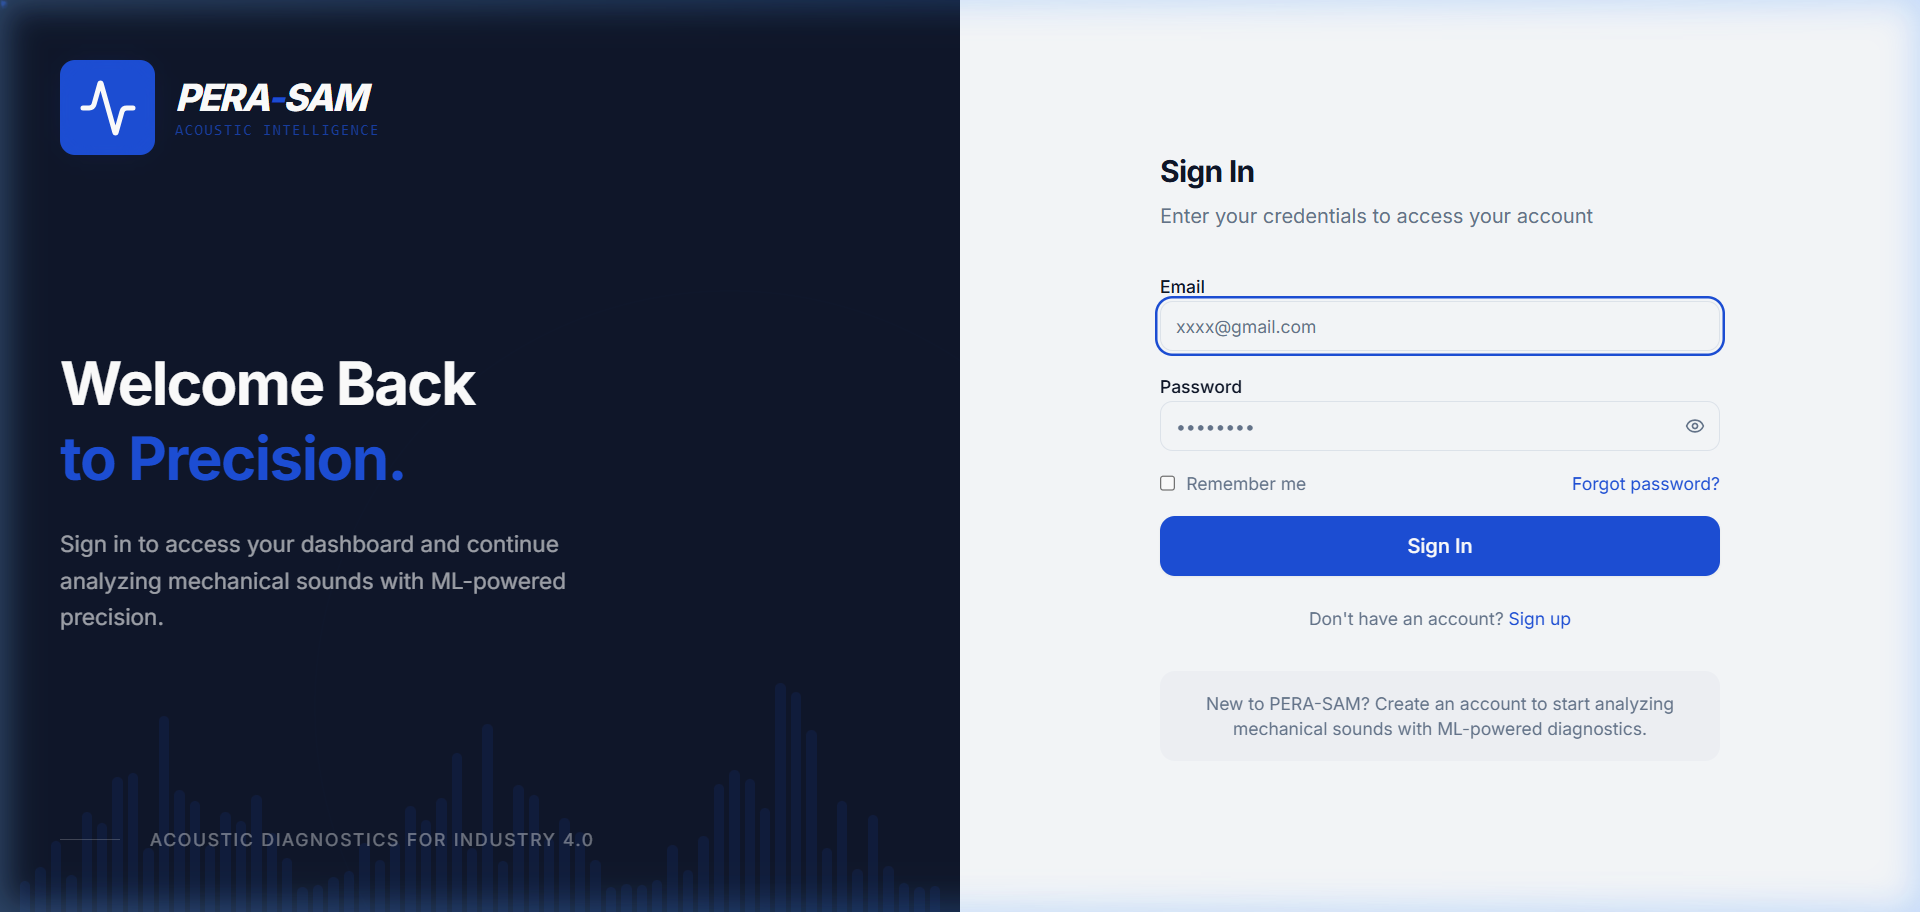
\includegraphics[width=0.60\textwidth]{login_page.png}
\caption{PERA-SAM Login Screen --- Web Application}
\label{fig:login-page}
\end{figure}

\begin{table}[H]
\centering
\caption{Login Screen Elements}
\label{tab:login-elements}
\begin{tabularx}{\textwidth}{l X}
  \toprule
  \textbf{Element} & \textbf{Description} \\
  \midrule
  Email Field          & Enter your registered email address. \\
  Password Field       & Enter your account password. \\
  Show/Hide Password   & Toggle button (eye icon) to reveal or conceal the password. \\
  Remember Me          & Checkbox to persist the session across app restarts. \\
  Sign In Button       & Submits the login credentials for authentication. \\
  Create Account Link  & Navigates to the Registration screen. \\
  Demo Mode Banner     & Displayed when Supabase is not configured; any credentials are accepted. \\
  \bottomrule
\end{tabularx}
\end{table}

\subsection*{Procedure --- Logging In}
\begin{enumerate}[leftmargin=*, nosep]
  \item Enter your \textbf{email address} in the Email field.
  \item Enter your \textbf{password} in the Password field.
  \item Optionally, check \textbf{Remember Me}.
  \item Tap \textbf{Sign In}.
  \item Upon successful authentication, you are redirected to the \textbf{Dashboard}.
\end{enumerate}

\subsection*{Error Handling}
\begin{table}[H]
\centering
\caption{Login Error Messages}
\label{tab:login-errors}
\begin{tabularx}{\textwidth}{l l X}
  \toprule
  \textbf{Error} & \textbf{Cause} & \textbf{Resolution} \\
  \midrule
  ``Missing Fields''         & Email or password is empty      & Fill in both fields \\
  ``Login Failed''           & Invalid credentials             & Check your email and password \\
  ``Network request failed'' & Cannot reach Supabase           & Check internet connection \\
  \bottomrule
\end{tabularx}
\end{table}

\section{Registration Screen}
\label{sec:registration}

New users must register before using the system.

\begin{table}[H]
\centering
\caption{Registration Screen Elements}
\label{tab:reg-elements}
\begin{tabularx}{\textwidth}{l X}
  \toprule
  \textbf{Element} & \textbf{Description} \\
  \midrule
  Full Name Field         & Your display name used across the application. \\
  Email Field             & Must be a valid email address. \\
  Password Field          & Minimum 6 characters. A strength indicator bar provides visual feedback. \\
  Confirm Password Field  & Must exactly match the password. \\
  Password Strength Bar   & Color-coded bar: Red ($<$ 6 chars), Amber (6--7 chars), Green (8+ chars). \\
  Create Account Button   & Submits the registration form. \\
  Sign In Link            & Returns to the Login screen. \\
  \bottomrule
\end{tabularx}
\end{table}

\subsection*{Procedure --- Creating an Account}
\begin{enumerate}[leftmargin=*, nosep]
  \item Enter your \textbf{Full Name}.
  \item Enter your \textbf{Email Address}.
  \item Enter a \textbf{Password} (minimum 6 characters). Observe the strength indicator.
  \item Re-enter your password in the \textbf{Confirm Password} field.
  \item Tap \textbf{Create Account}.
  \item Check your email inbox for a \textbf{confirmation link} (if Supabase email verification is enabled).
  \item After confirming, return to the Login screen and sign in.
\end{enumerate}

\section{Dashboard (Home)}
\label{sec:dashboard}

The Dashboard is the primary screen after login, providing a real-time overview of machine health status. Figure~\ref{fig:dashboard-page} shows the web dashboard with analysis summary cards, recent analyses, quick actions, and AI system status.

\begin{figure}[H]
\centering
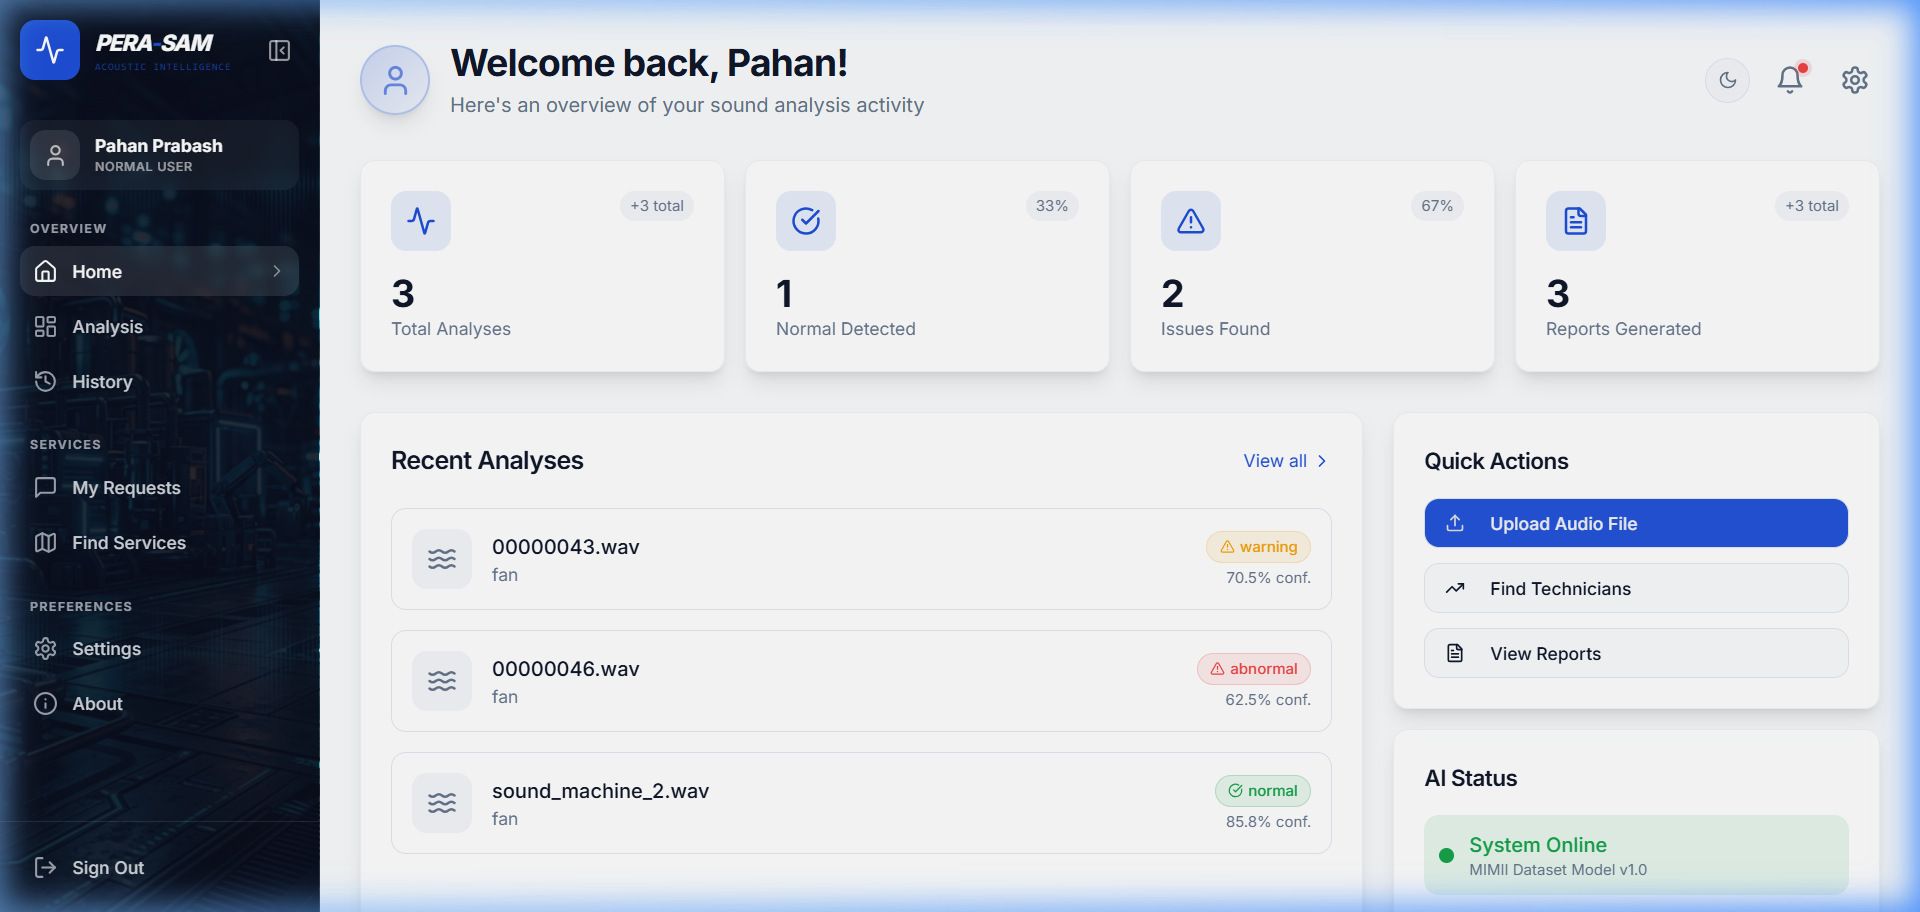
\includegraphics[width=0.62\textwidth]{dashboard_page.png}
\caption{PERA-SAM Dashboard --- Overview of Sound Analysis Activity}
\label{fig:dashboard-page}
\end{figure}

\begin{table}[H]
\centering
\caption{Dashboard Elements}
\label{tab:dashboard-elements}
\begin{tabularx}{\textwidth}{l X}
  \toprule
  \textbf{Element} & \textbf{Description} \\
  \midrule
  Greeting Header    & Displays ``Hello, [Name]'' with a personalized welcome. \\
  Notification Bell  & Opens the notification modal showing recent alerts. \\
  Quick Actions Card & Shortcut to ``Start Analysis'' and ``View History''. \\
  Recent Analyses    & List of the 5 most recent analysis records with status indicators. \\
  Pull-to-Refresh    & Swipe down to reload dashboard data. \\
  \bottomrule
\end{tabularx}
\end{table}

\begin{table}[H]
\centering
\caption{Notification Types}
\label{tab:notifications}
\begin{tabularx}{\textwidth}{l l X}
  \toprule
  \textbf{Type} & \textbf{Icon} & \textbf{Description} \\
  \midrule
  Anomaly Alert  & \ding{43} & A recent analysis detected an anomaly or warning condition. \\
  Message        & \ding{46} & New chat message from a service provider. \\
  Repair Update  & \ding{80} & Status change on a repair request. \\
  System         & \ding{46} & General system notifications. \\
  \bottomrule
\end{tabularx}
\end{table}

\section{Analysis Screen}
\label{sec:analysis}

The Analysis Screen is the core feature of PERA-SAM, where users submit audio samples for anomaly detection. Figure~\ref{fig:analysis-page} shows the web-based analysis interface with audio upload, equipment details, and the Analyze Sound button.

\begin{figure}[H]
\centering
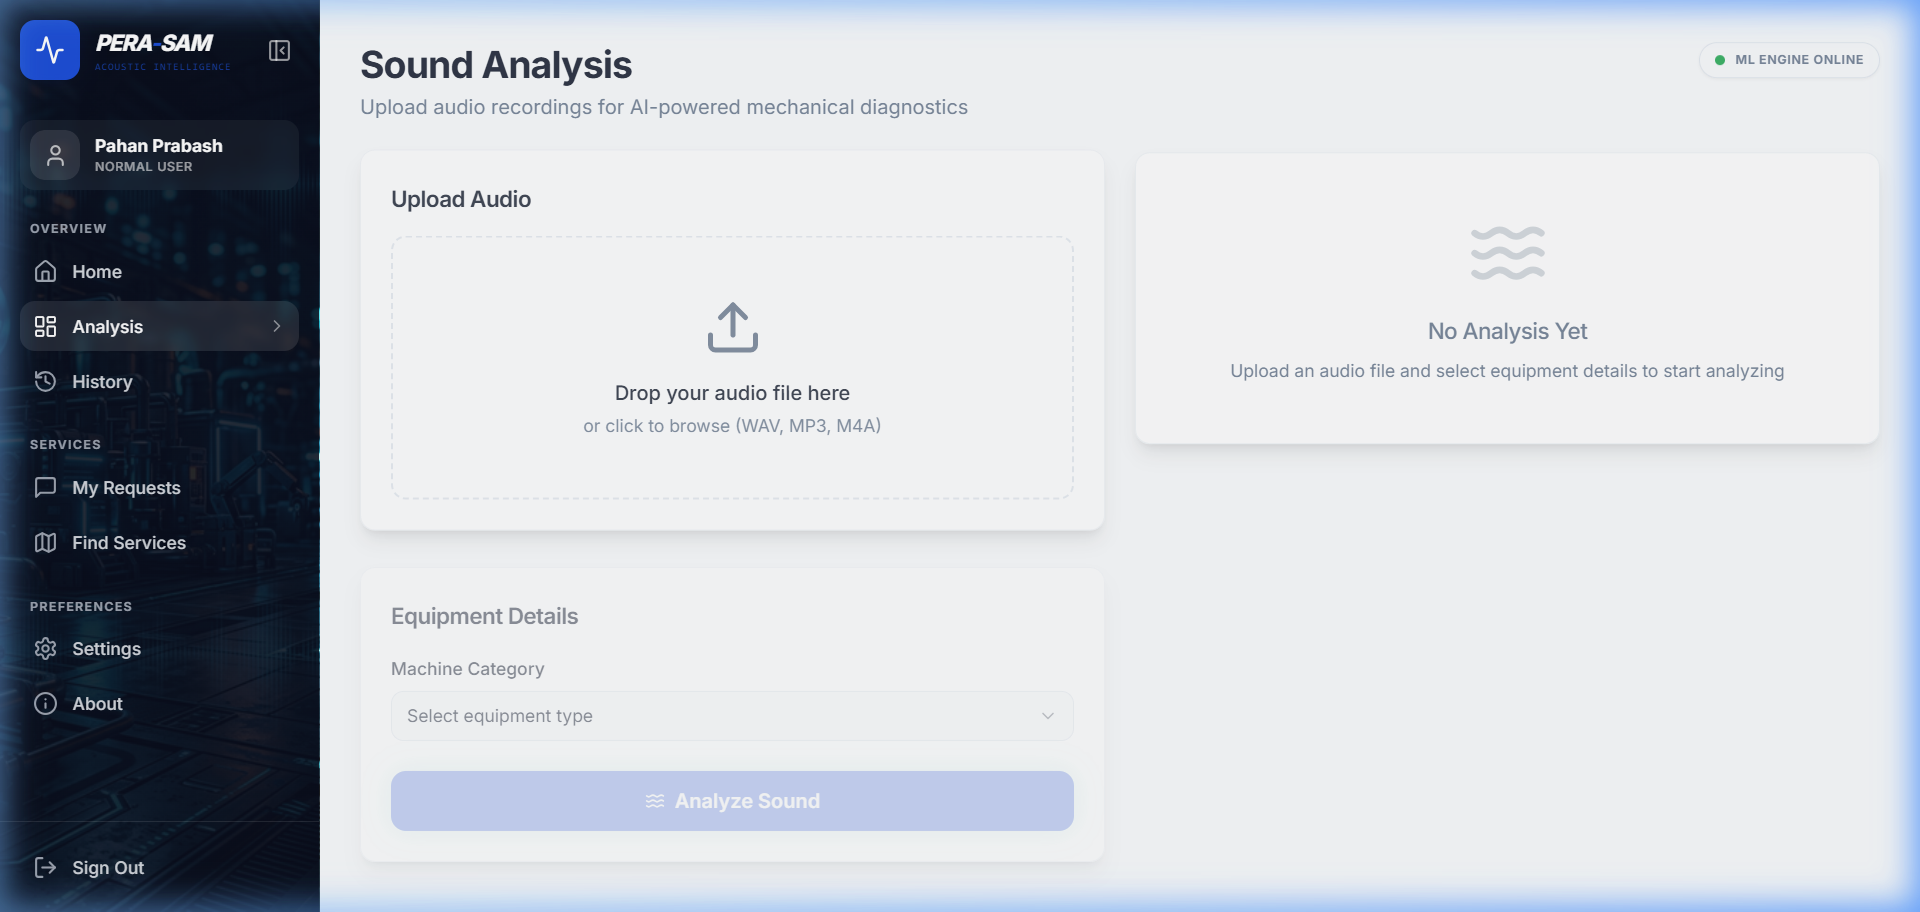
\includegraphics[width=0.62\textwidth]{analysis_page.png}
\caption{PERA-SAM Sound Analysis Screen --- Audio Upload and Equipment Selection}
\label{fig:analysis-page}
\end{figure}

\begin{table}[H]
\centering
\caption{Analysis Screen Elements}
\label{tab:analysis-elements}
\begin{tabularx}{\textwidth}{l X}
  \toprule
  \textbf{Element} & \textbf{Description} \\
  \midrule
  Machine Category Selector & Choose the machine type: Fan, Pump, Slider, Valve, or Vehicle Bearing. \\
  Upload Audio Button       & Opens the device file picker to select a \texttt{.wav} audio file. \\
  Record Audio Button       & Starts/stops live audio recording using the device microphone. \\
  Recording Indicator       & Pulsing red dot and timer displayed during active recording. \\
  Selected File Info        & Shows filename, size, and source of the selected audio. \\
  Analyze Button            & Sends the selected audio to the ML Backend for processing. \\
  Results Panel             & Displays the analysis outcome after processing. \\
  Save to History Button    & Persists the result to the analysis history in Supabase. \\
  \bottomrule
\end{tabularx}
\end{table}

\subsection*{Procedure --- Analyzing Machine Sound}
\begin{enumerate}[leftmargin=*, nosep]
  \item Navigate to the \textbf{Analysis} tab (microphone icon in the bottom bar).
  \item \textbf{Select a Machine Category} from the horizontal category list.
  \item Provide audio input via one of two methods:
  \begin{itemize}
    \item \textbf{Method A --- Upload:} Tap \textbf{Upload Audio File}. Select a \texttt{.wav} file from your device storage.
    \item \textbf{Method B --- Record:} Tap \textbf{Record Audio}. Grant microphone permission. Position the device near the machine. Tap \textbf{Stop Recording} when sufficient audio is captured.
  \end{itemize}
  \item Tap the \textbf{Analyze} button.
  \item Wait for the analysis to complete (a loading spinner is displayed).
  \item Review the results (see Table~\ref{tab:status-colors}).
  \item Optionally tap \textbf{Save to History} to persist the result.
\end{enumerate}

\begin{table}[H]
\centering
\caption{Status Color Interpretation}
\label{tab:status-colors}
\begin{tabularx}{\textwidth}{l l X}
  \toprule
  \textbf{Status} & \textbf{Color} & \textbf{Meaning} \\
  \midrule
  \ding{51} Normal  & \textcolor{successgreen}{Green} & Machine operating within normal parameters. No action required. \\
  \ding{43} Warning & \textcolor{warningamber}{Amber}  & Unusual patterns detected. Schedule maintenance soon. \\
  \ding{54} Anomaly & \textcolor{dangerred}{Red}       & Machine failure may be imminent. Stop operation and inspect immediately. \\
  \bottomrule
\end{tabularx}
\end{table}

\section{Web Dashboard --- Sound Analysis Interface}
\label{sec:web-analysis}

The web dashboard provides the same analysis capabilities with a richer visual interface. Figure~\ref{fig:analysis-screens} shows the three possible analysis outcomes.

\begin{figure}[H]
\centering
\begin{subfigure}[b]{0.48\textwidth}
  \centering
  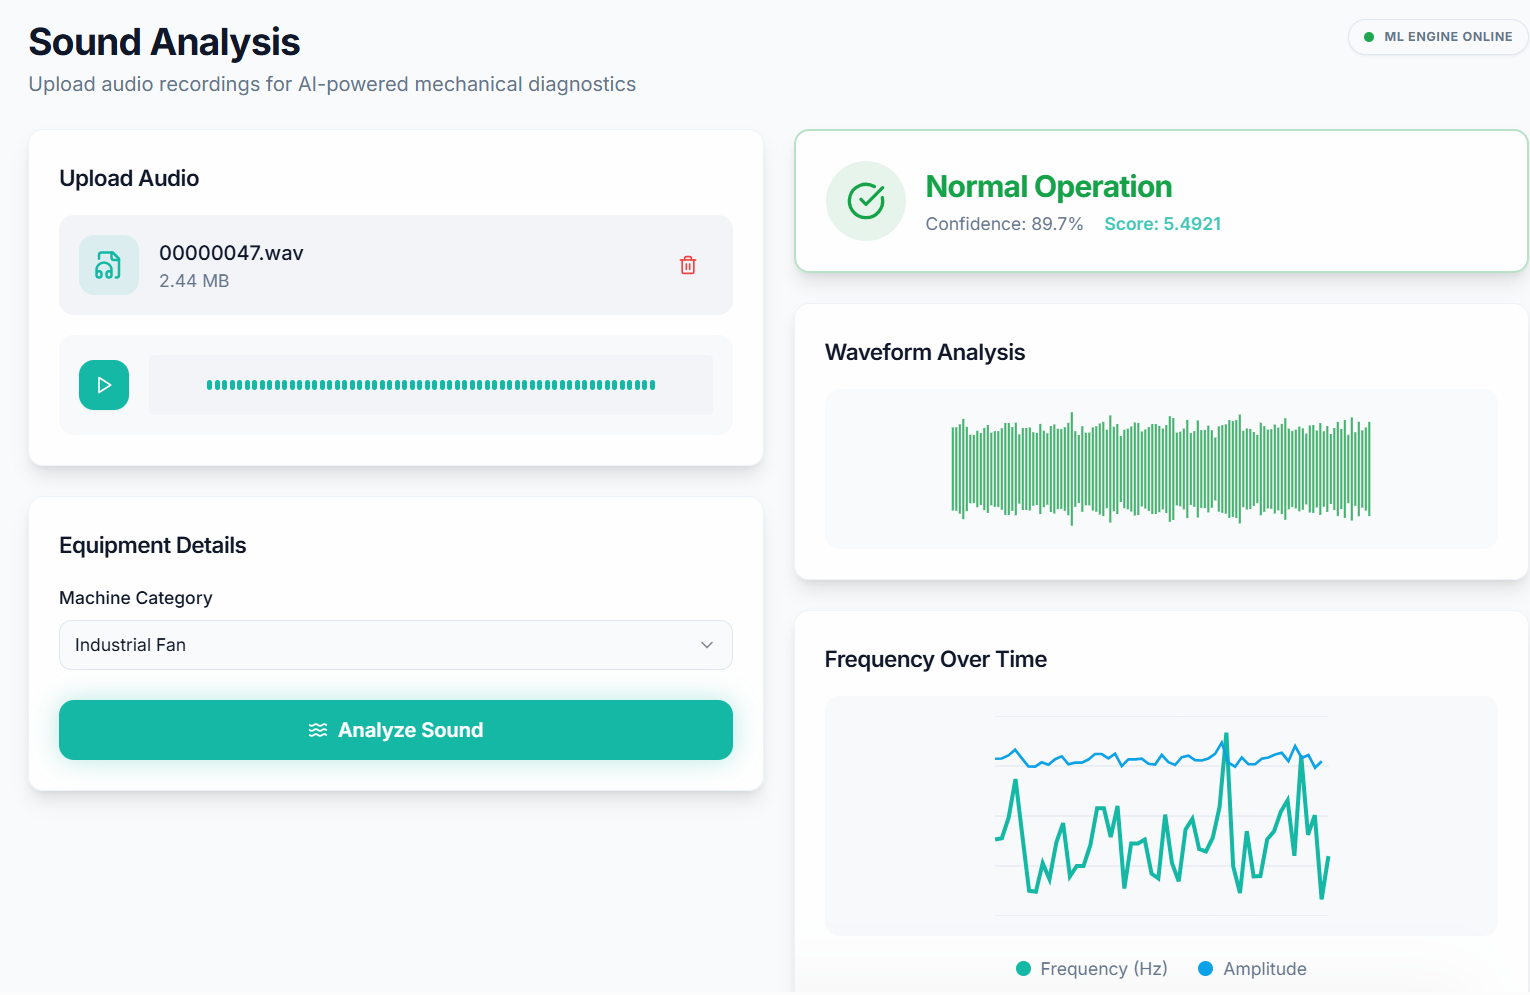
\includegraphics[width=0.92\linewidth]{Test5.png}
  \caption{Normal Operation --- Health score 89.7\%}
  \label{fig:normal}
\end{subfigure}
\hfill
\begin{subfigure}[b]{0.48\textwidth}
  \centering
  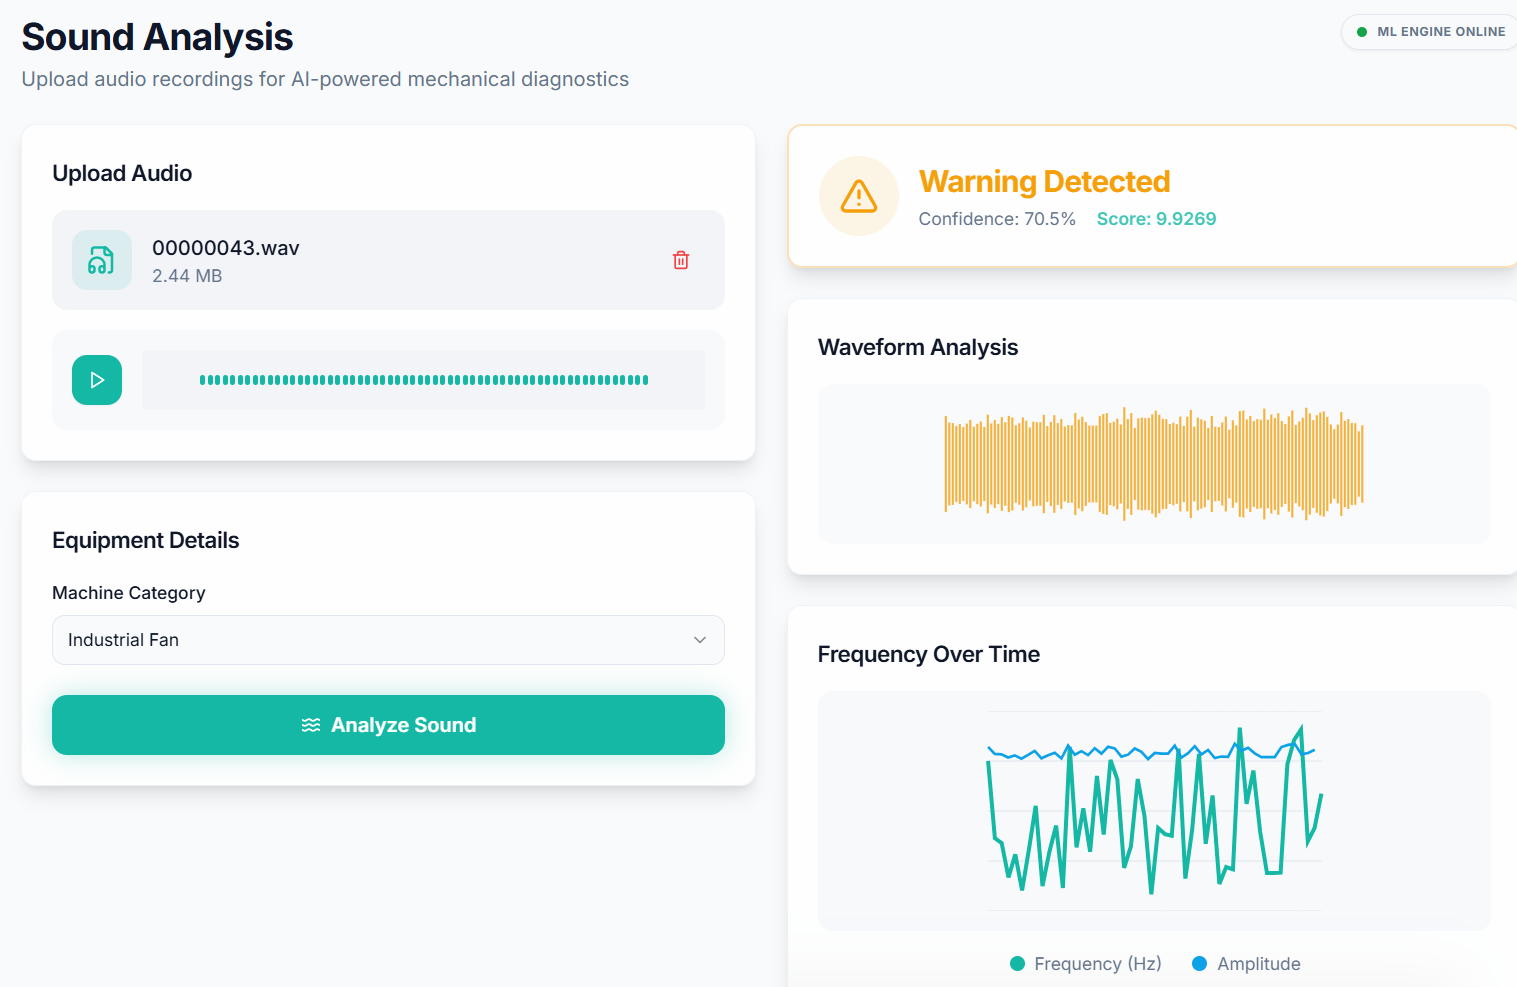
\includegraphics[width=0.92\linewidth]{Test1.png}
  \caption{Warning Detected --- Confidence 70.5\%}
  \label{fig:warning}
\end{subfigure}

\vspace{0.15cm}

\begin{subfigure}[b]{0.48\textwidth}
  \centering
  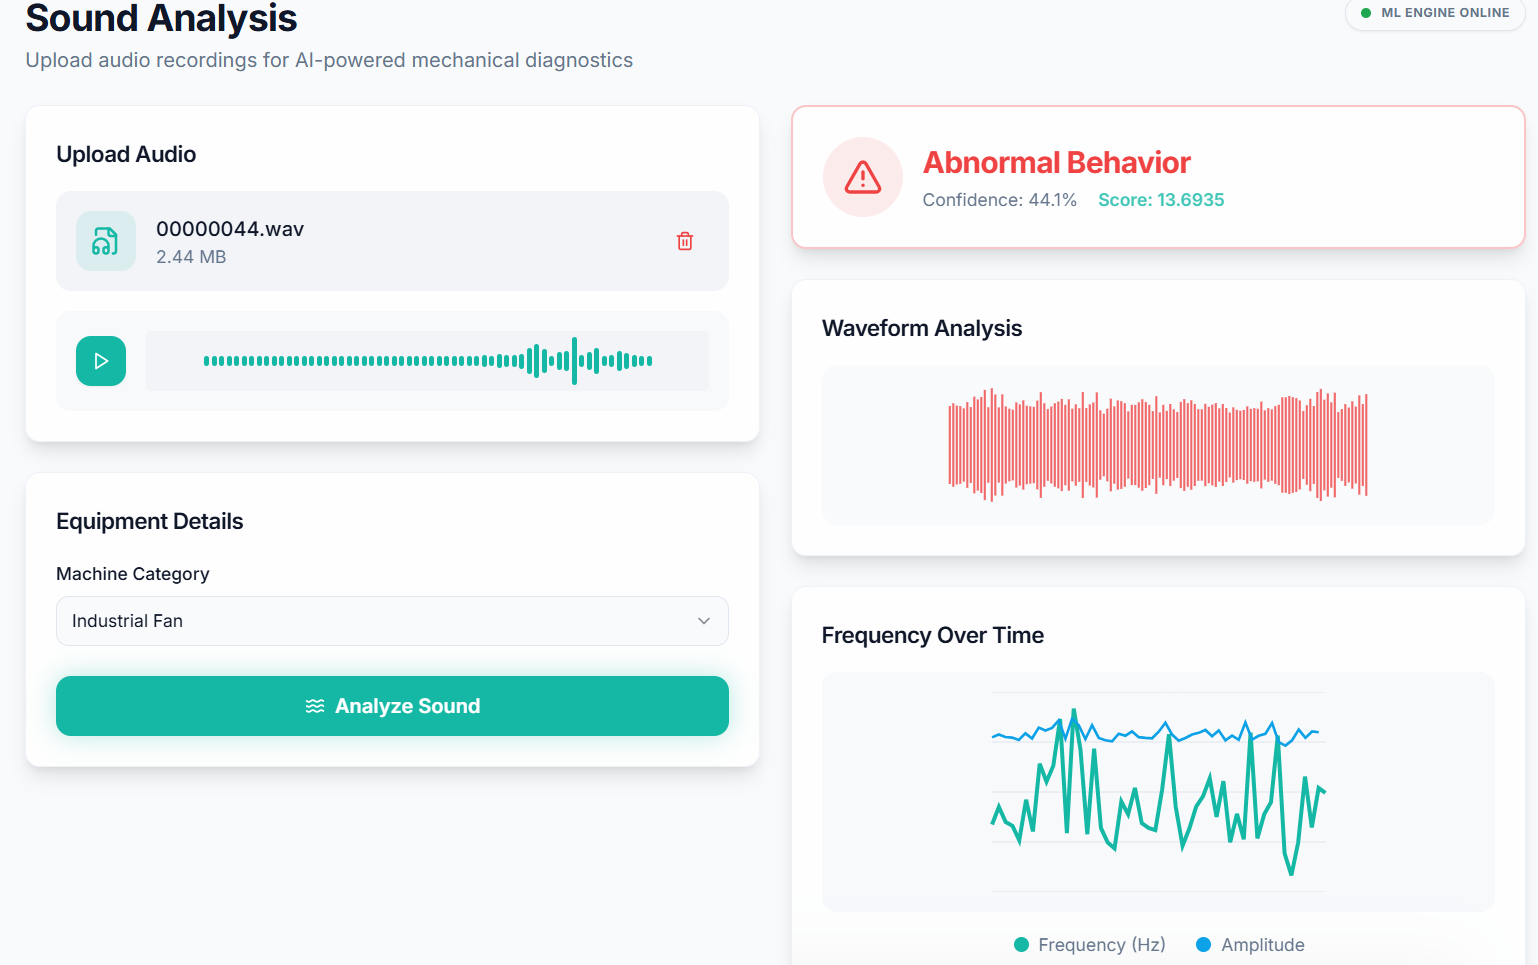
\includegraphics[width=0.92\linewidth]{Test2.png}
  \caption{Abnormal Behavior --- Confidence 44.1\%}
  \label{fig:anomaly}
\end{subfigure}
\hfill
\begin{subfigure}[b]{0.48\textwidth}
  \centering
  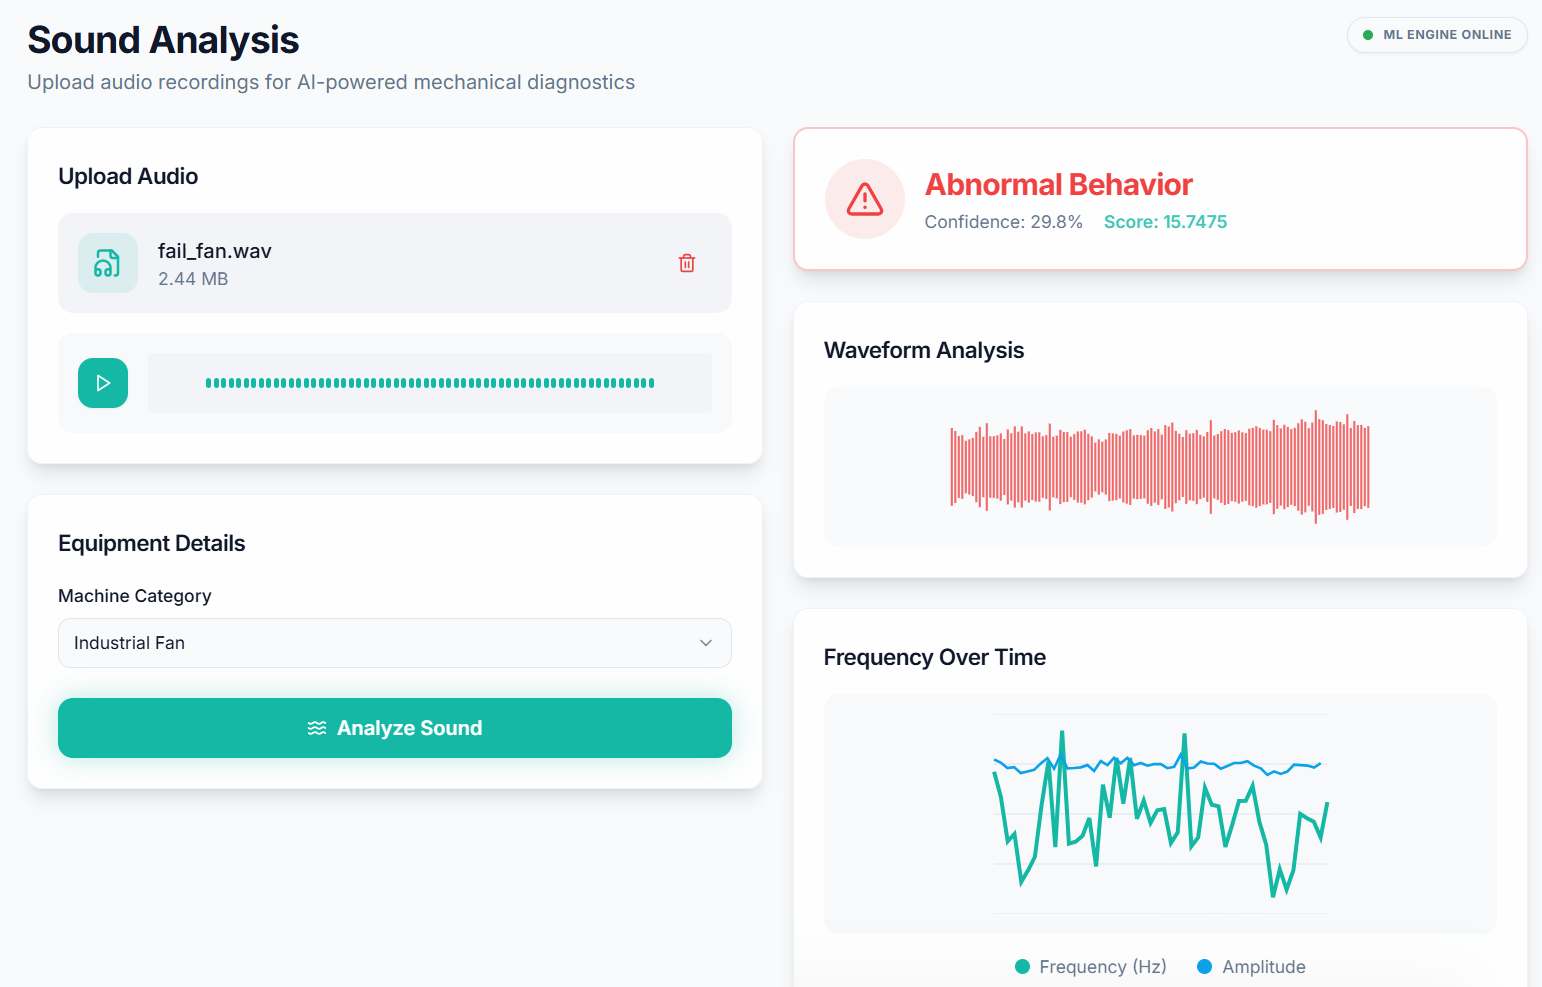
\includegraphics[width=0.92\linewidth]{Test8.png}
  \caption{Abnormal Behavior --- fail\_fan.wav}
  \label{fig:anomaly-fail}
\end{subfigure}
\caption{Web Dashboard --- Sound Analysis Results}
\label{fig:analysis-screens}
\end{figure}

\section{Map --- Service Providers}
\label{sec:map}

The Map screen helps users discover nearby repair and maintenance service providers. Figure~\ref{fig:services-page} shows the Find Services interface with an interactive map, category filters, and a list of nearby service providers with ratings.

\begin{figure}[H]
\centering
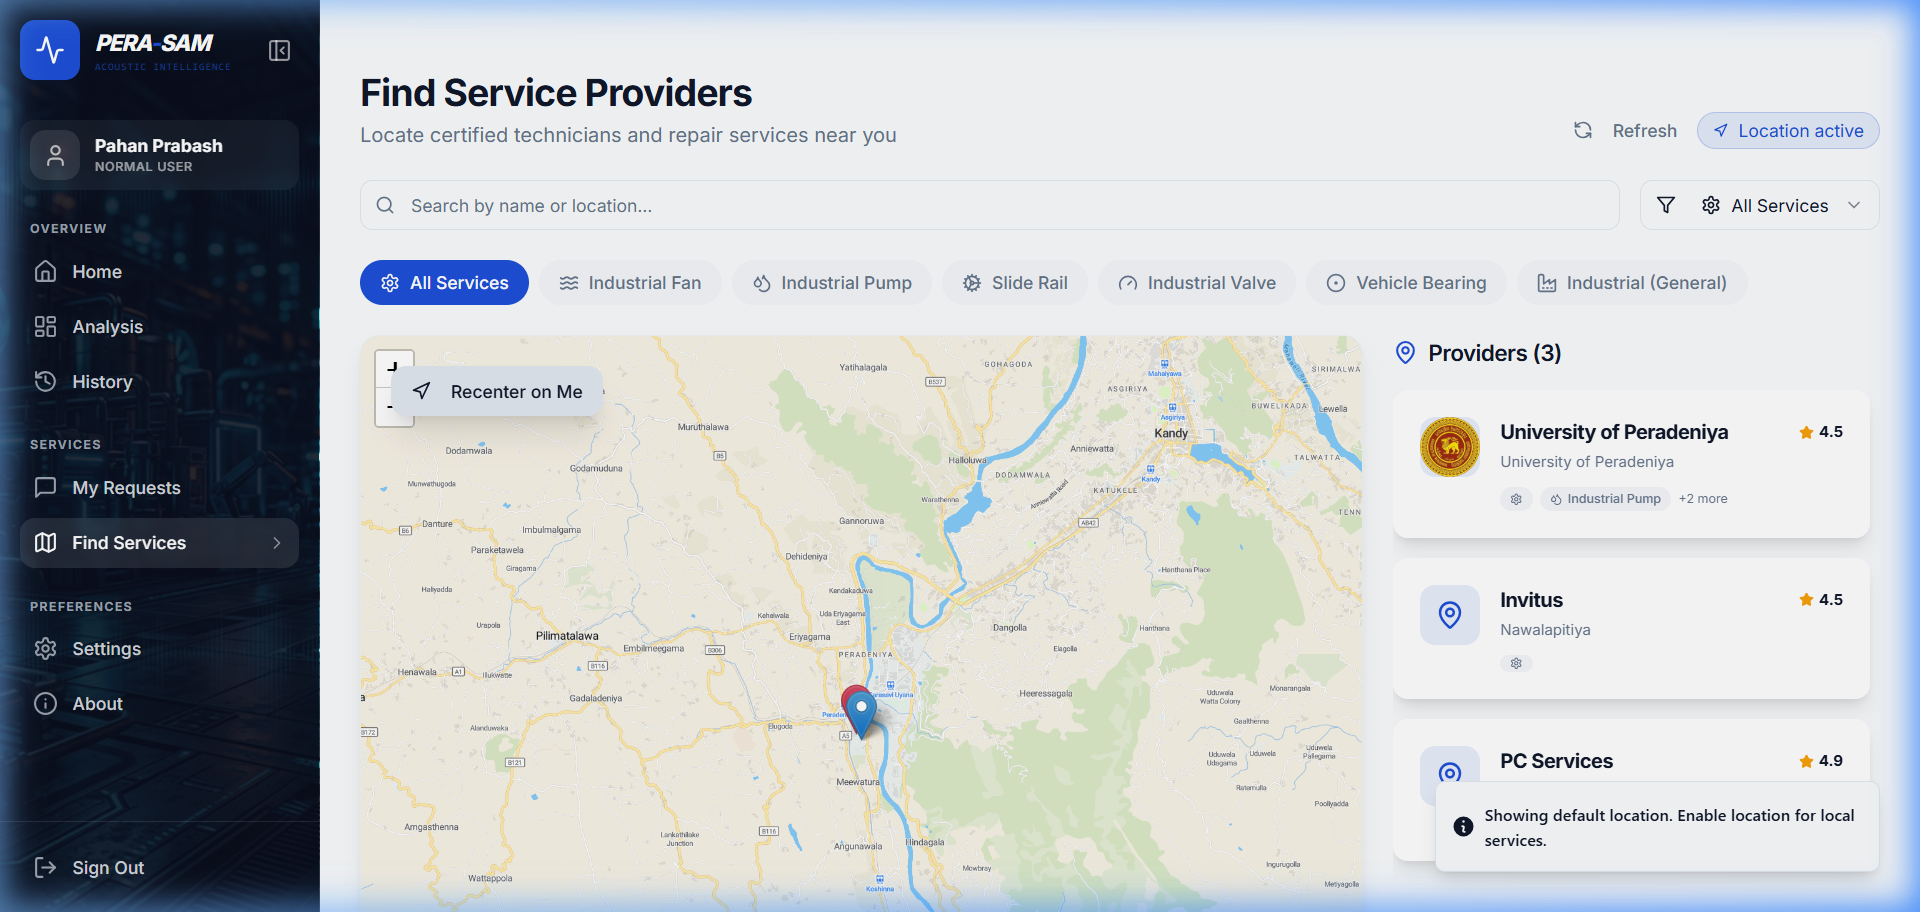
\includegraphics[width=0.62\textwidth]{services_page.png}
\caption{PERA-SAM Find Service Providers --- Map View with Provider Listings}
\label{fig:services-page}
\end{figure}

\begin{table}[H]
\centering
\caption{Map Screen Elements}
\label{tab:map-elements}
\begin{tabularx}{\textwidth}{l X}
  \toprule
  \textbf{Element} & \textbf{Description} \\
  \midrule
  Search Bar          & Search service providers by name or keyword. \\
  Category Filters    & Horizontal filter chips: All, Fan, Pump, Slider, Valve, Bearing, General. \\
  Provider List       & Scrollable list of service providers sorted by distance. \\
  Provider Card       & Displays name, address, rating, distance, availability, and contact. \\
  Request Repair      & Initiates a repair request to the selected provider. \\
  Call Button         & Opens the phone dialer with the provider's number. \\
  Get Directions      & Opens the native maps app with directions. \\
  \bottomrule
\end{tabularx}
\end{table}

\section{Repair Requests}
\label{sec:requests}

The Requests screen manages the lifecycle of repair requests between users and service providers.

\subsection*{Request Status Lifecycle}

\begin{figure}[H]
\centering
\begin{tikzpicture}[
  state/.style={draw, rounded corners=4pt, minimum width=2.5cm, minimum height=1cm,
                align=center, font=\small\bfseries},
  arrow/.style={->, thick, >=stealth},
  label/.style={font=\footnotesize, midway, above}
]
  \node[state, fill=warningamber!20] (pending) at (0, 0) {Pending};
  \node[state, fill=ieeeblue!20]    (accepted) at (4.5, 0) {Accepted};
  \node[state, fill=successgreen!20] (completed) at (9, 0) {Completed};
  \node[state, fill=dangerred!20]   (declined) at (0, -2) {Declined};

  \draw[arrow] (pending)  -- node[label] {Accept}   (accepted);
  \draw[arrow] (accepted) -- node[label] {Complete}  (completed);
  \draw[arrow] (pending)  -- node[label, left] {Decline} (declined);
\end{tikzpicture}
\caption{Repair Request Status Lifecycle}
\label{fig:request-lifecycle}
\end{figure}

\begin{table}[H]
\centering
\caption{Request Status Meanings}
\label{tab:request-status}
\begin{tabularx}{\textwidth}{l l X}
  \toprule
  \textbf{Status} & \textbf{Color} & \textbf{Description} \\
  \midrule
  Pending   & \textcolor{warningamber}{Amber} & Request submitted; awaiting provider response. \\
  Accepted  & \textcolor{ieeeblue}{Blue}      & Provider has accepted and work is in progress. \\
  Completed & \textcolor{successgreen}{Green}  & Repair has been completed successfully. \\
  Declined  & \textcolor{dangerred}{Red}       & Provider has declined the request. \\
  \bottomrule
\end{tabularx}
\end{table}

\section{Chat --- Real-Time Messaging}
\label{sec:chat}

The Chat screen provides real-time communication between users and service providers within the context of a repair request.

Features:
\begin{itemize}[leftmargin=*, nosep]
  \item Messages are \textbf{color-coded} by sender (your messages on the right in indigo, received messages on the left in white).
  \item \textbf{Real-time updates} via Supabase PostgreSQL change subscriptions.
  \item \textbf{Read status tracking} for unread message indicators.
  \item \textbf{Unread badge} on the Requests tab icon showing the count of unread messages.
\end{itemize}

\subsection*{Procedure --- Sending a Message}
\begin{enumerate}[leftmargin=*, nosep]
  \item From the \textbf{Requests} screen, tap the \textbf{Chat} button on any request.
  \item Type your message in the input field at the bottom.
  \item Tap the \textbf{Send} button (paper plane icon).
  \item The message appears instantly in the conversation.
\end{enumerate}

\section{Analysis History}
\label{sec:history}

The History screen provides a comprehensive log of all past analyses performed by the user. Figure~\ref{fig:history-page} shows the analysis history with summary statistics, search/filter capabilities, and individual analysis records with status badges.

\begin{figure}[H]
\centering
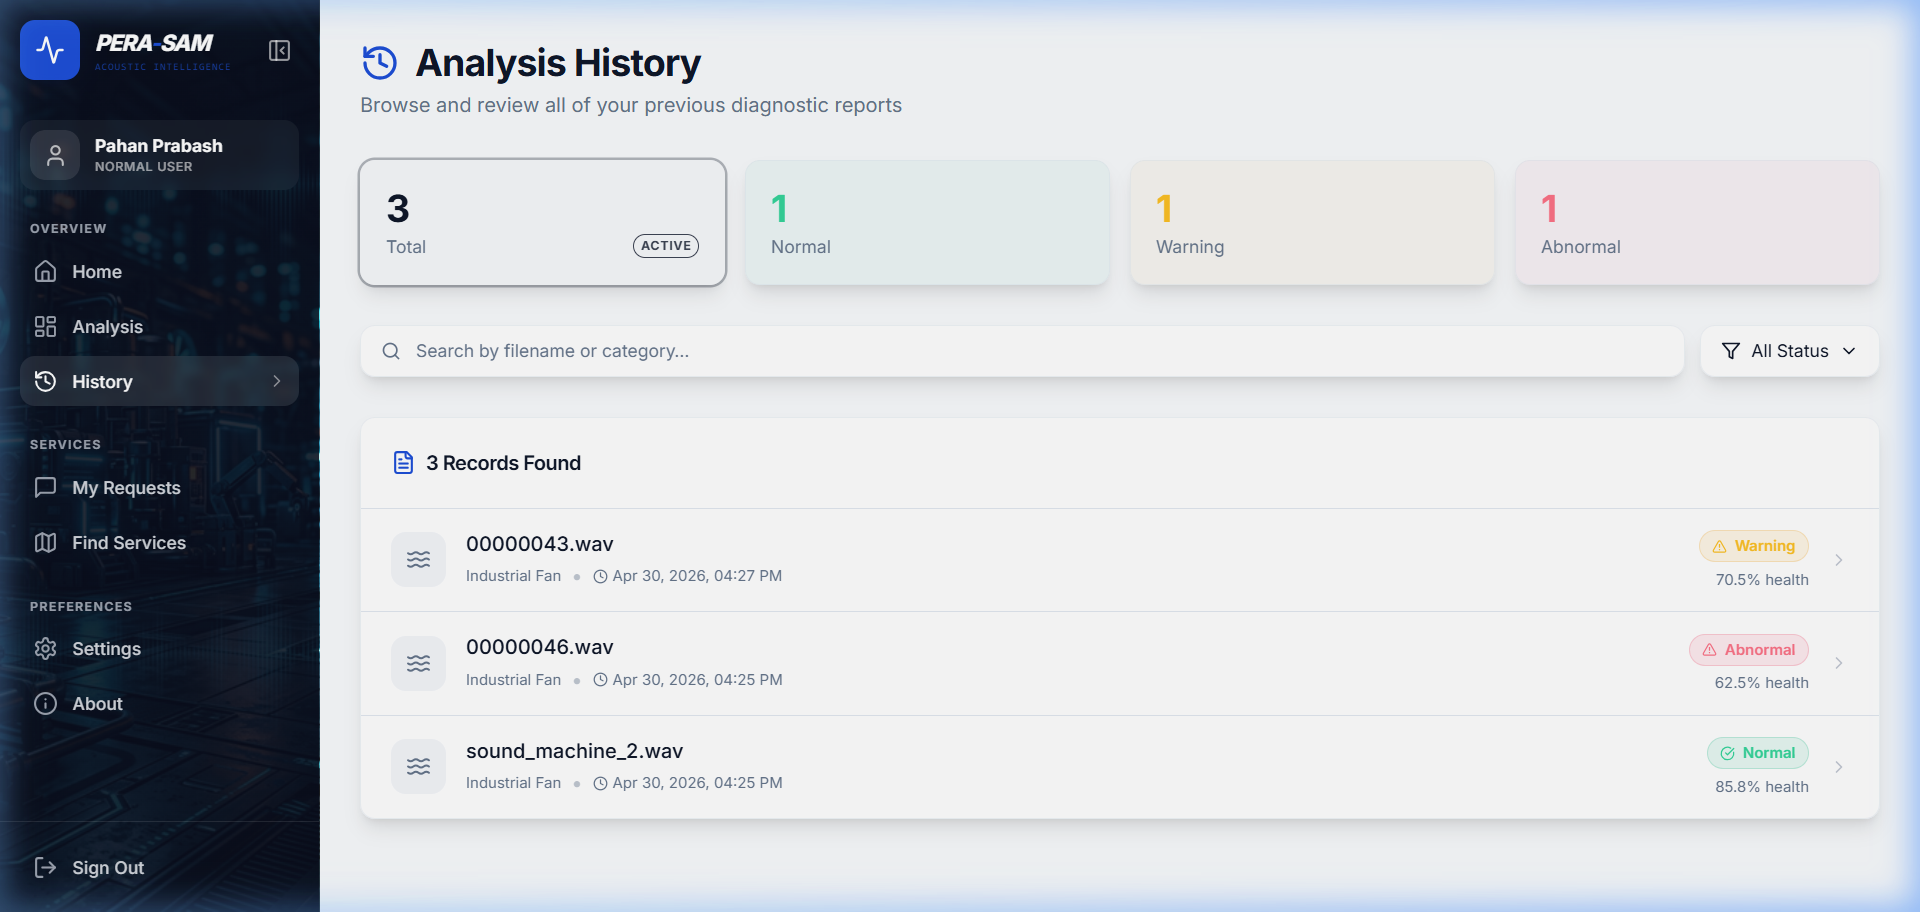
\includegraphics[width=0.62\textwidth]{history_page.png}
\caption{PERA-SAM Analysis History --- Browsing Previous Diagnostic Reports}
\label{fig:history-page}
\end{figure}

\begin{table}[H]
\centering
\caption{Analysis History Detail Fields}
\label{tab:history-fields}
\begin{tabularx}{\textwidth}{l X}
  \toprule
  \textbf{Field} & \textbf{Description} \\
  \midrule
  Category       & Machine type analyzed \\
  Machine ID     & Specific machine model matched \\
  Status         & Normal / Warning / Anomaly \\
  Confidence     & Model prediction confidence percentage \\
  Anomaly Score  & Raw reconstruction error value \\
  Recommendation & Suggested action based on the analysis \\
  Filename       & Original audio file name \\
  Analyzed On    & Timestamp of the analysis \\
  \bottomrule
\end{tabularx}
\end{table}

\section{Profile Screen}
\label{sec:profile}

The Profile screen displays user account information, system configuration status, and technology stack details.

\begin{table}[H]
\centering
\caption{System Status Indicators}
\label{tab:system-status}
\begin{tabularx}{\textwidth}{l l X}
  \toprule
  \textbf{Indicator} & \textbf{Color} & \textbf{Meaning} \\
  \midrule
  \ding{51} Connected & \textcolor{successgreen}{Green} & Service is reachable and configured. \\
  \ding{43} Demo Mode & \textcolor{warningamber}{Amber}  & Supabase not configured; using mock data. \\
  \ding{54} Error     & \textcolor{dangerred}{Red}       & Service is unreachable or misconfigured. \\
  \bottomrule
\end{tabularx}
\end{table}


% ══════════════════════════════════════════════════════════════════════════════
%  CHAPTER 5 — ML BACKEND API
% ══════════════════════════════════════════════════════════════════════════════
\chapter{Using the Software --- ML Backend API}
\label{ch:api}

\section{API Overview}
\label{sec:api-overview}

The PERA-SAM ML Backend exposes a RESTful API built with FastAPI. It provides endpoints for health checking, model listing, and audio analysis.

\begin{itemize}[leftmargin=*, nosep]
  \item \textbf{Base URL:} \texttt{http://<host>:8000}
  \item \textbf{Authentication:} The API currently does not require authentication. Access control should be managed at the network level.
  \item \textbf{Request Content-Type:} \texttt{multipart/form-data} (for file uploads)
  \item \textbf{Response Content-Type:} \texttt{application/json}
\end{itemize}

\section{Endpoints Reference}
\label{sec:endpoints}

\subsection{GET \texttt{/} --- API Status}

Returns the current status of the ML backend.

\begin{lstlisting}[caption={API Status --- Request and Response}]
GET http://localhost:8000/

Response:
{
  "status": "Online",
  "message": "PERA-SAM ML Sound Analysis API",
  "version": "2.0.0",
  "models_loaded": 6,
  "capabilities": [
    "Auto-Train on Startup",
    "Anomaly Detection",
    "Per-Model Calibrated Thresholds",
    "Health Scoring",
    "Multi-Machine Identification"
  ]
}
\end{lstlisting}

\subsection{GET \texttt{/health} --- Health Check}

\begin{lstlisting}[caption={Health Check Endpoint}]
GET http://localhost:8000/health

Response: { "status": "ok" }
\end{lstlisting}

\subsection{GET \texttt{/models} --- Available Models}

\begin{lstlisting}[caption={Models Endpoint}]
GET http://localhost:8000/models

Response:
{
  "categories": {
    "fan":    ["00", "02", "04", "06"],
    "pump":   ["00", "02", "04", "06"],
    "slider": ["00", "02", "04", "06"],
    "valve":  ["00", "02", "04", "06"]
  },
  "metrics_available": [...]
}
\end{lstlisting}

\subsection{POST \texttt{/analyze} --- Analyze Audio File}

The primary endpoint. Uploads a WAV audio file and receives an anomaly detection result.

\begin{lstlisting}[caption={Analyze Endpoint --- Request}]
POST http://localhost:8000/analyze
Content-Type: multipart/form-data

Fields:
  file: (binary)     -- Required. The WAV audio file.
  category: string   -- Optional. Machine category.
  machine_id: string -- Optional. Specific machine ID.
\end{lstlisting}

Example using cURL:
\begin{lstlisting}[language=bash, caption={cURL example}]
> curl -X POST http://localhost:8000/analyze \
    -F "file=@machine_recording.wav" \
    -F "category=fan" \
    -F "machine_id=00"
\end{lstlisting}

\begin{table}[H]
\centering
\caption{Analysis Modes}
\label{tab:analysis-modes}
\begin{tabularx}{\textwidth}{l l X}
  \toprule
  \textbf{Mode} & \textbf{Condition} & \textbf{Behavior} \\
  \midrule
  Direct Mode      & Both \texttt{category} and \texttt{machine\_id} provided & Uses the specified model with its calibrated threshold \\
  Auto-Detect Mode & Only \texttt{category} provided & Scans all models in the category; picks the best match \\
  Default Mode     & Neither provided & Falls back to a general-purpose default model \\
  \bottomrule
\end{tabularx}
\end{table}

\section{Interpreting Analysis Results}
\label{sec:interpret-results}

\subsection{Status Classification}

The system classifies the result into one of three statuses based on the anomaly score relative to the calibrated threshold:

\begin{table}[H]
\centering
\caption{Status Classification Rules}
\label{tab:status-rules}
\begin{tabularx}{\textwidth}{l l X}
  \toprule
  \textbf{Status} & \textbf{Condition} & \textbf{Meaning} \\
  \midrule
  Normal  & $\text{score} < \text{threshold} \times 0.8$                                       & Machine operating within normal parameters. \\
  Warning & $\text{threshold} \times 0.8 \leq \text{score} \leq \text{threshold}$               & Unusual patterns detected; degradation beginning. \\
  Anomaly & $\text{score} > \text{threshold}$                                                   & Significant deviation from normal; potential failure. \\
  \bottomrule
\end{tabularx}
\end{table}

\subsection{Key Metrics Explained}

\begin{table}[H]
\centering
\caption{Analysis Metrics}
\label{tab:metrics}
\begin{tabularx}{\textwidth}{l l X}
  \toprule
  \textbf{Metric} & \textbf{Range} & \textbf{Description} \\
  \midrule
  \texttt{score}                & $0 - \infty$  & Mean Squared Error between input and autoencoder reconstruction. Lower is healthier. \\
  \texttt{max\_frame\_error}    & $0 - \infty$  & Maximum per-frame MSE. High values indicate transient spikes. \\
  \texttt{min\_frame\_error}    & $0 - \infty$  & Minimum per-frame MSE. Represents the ``cleanest'' portion. \\
  \texttt{threshold\_used}      & $0 - \infty$  & The calibrated decision boundary. \\
  \texttt{health\_percentage}   & $0 - 100$     & Human-readable health score. \\
  \texttt{model\_auc}           & $0 - 1.0$     & Area Under the Curve. Higher = more reliable. \\
  \texttt{detection\_reliability} & Text         & High (AUC $> 0.85$), Medium ($0.7$--$0.85$), Low ($< 0.7$). \\
  \bottomrule
\end{tabularx}
\end{table}

\section{Health Scoring System}
\label{sec:health-scoring}

The health percentage is calculated as follows:

\begin{table}[H]
\centering
\caption{Health Scoring Formulas}
\label{tab:health-formulas}
\begin{tabularx}{\textwidth}{l X l}
  \toprule
  \textbf{Condition} & \textbf{Formula} & \textbf{Health Range} \\
  \midrule
  $s < T \times 0.8$              & $100 - \frac{s}{T \times 0.8} \times 15$                          & 85\%--100\% \\[6pt]
  $T \times 0.8 \leq s \leq T$   & $85 - \frac{s - T \times 0.8}{T \times 0.2} \times 15$            & 70\%--85\%  \\[6pt]
  $s > T$                         & $\max\!\left(0,\; 70 - \frac{s - T}{T} \times 70\right)$          & 0\%--70\%   \\
  \bottomrule
\end{tabularx}
\end{table}

Where $s$ = anomaly score and $T$ = calibrated threshold.

\begin{table}[H]
\centering
\caption{Health Interpretation Guide}
\label{tab:health-guide}
\begin{tabularx}{\textwidth}{l l X}
  \toprule
  \textbf{Health \%} & \textbf{Engine Health} & \textbf{Recommended Action} \\
  \midrule
  85\%--100\% & Good      & No action needed. Continue normal operation. \\
  70\%--85\%  & Degrading & Schedule preventive maintenance within the next window. \\
  0\%--70\%   & Critical  & \textbf{URGENT:} Stop operation immediately. Inspect the machine. \\
  \bottomrule
\end{tabularx}
\end{table}


% ══════════════════════════════════════════════════════════════════════════════
%  CHAPTER 6 — ERROR MESSAGES AND TROUBLESHOOTING
% ══════════════════════════════════════════════════════════════════════════════
\chapter{Error Messages and Troubleshooting}
\label{ch:troubleshooting}

\section{Mobile Application Errors}

\begin{table}[H]
\centering
\caption{Mobile Application Errors}
\label{tab:mobile-errors}
\begin{tabularx}{\textwidth}{p{3.8cm} p{4.2cm} X}
  \toprule
  \textbf{Error Message} & \textbf{Probable Cause} & \textbf{Resolution} \\
  \midrule
  ``Missing Fields''         & Form fields are empty               & Fill in all required fields \\
  ``Weak Password''          & Password $<$ 6 characters           & Use $\geq$ 6 characters \\
  ``Password Mismatch''      & Confirm password mismatch           & Re-enter the confirmation password \\
  ``Login Failed''           & Invalid credentials                 & Verify email and password \\
  ``Network request failed'' & Supabase URL unreachable            & Check internet; verify \texttt{EXPO\_PUBLIC\_SUPABASE\_URL} \\
  ``ML API not configured''  & \texttt{EXPO\_PUBLIC\_ML\_API\_URL} missing & Add URL to \texttt{.env}; restart Expo \\
  ``Analysis failed''        & ML backend error                    & Check backend is running; verify audio file \\
  ``Audio too short''        & Insufficient audio duration         & Re-record or upload longer sample ($\geq$ 0.5s) \\
  \bottomrule
\end{tabularx}
\end{table}

\section{ML Backend Errors}

\begin{table}[H]
\centering
\caption{ML Backend Errors}
\label{tab:backend-errors}
\begin{tabularx}{\textwidth}{p{4.2cm} p{4.2cm} X}
  \toprule
  \textbf{Error / Log Message} & \textbf{Probable Cause} & \textbf{Resolution} \\
  \midrule
  \texttt{config.yaml not found}     & Configuration file missing     & Create \texttt{config.yaml} in \texttt{model/server/} \\
  \texttt{No .h5 models in assets/}  & No trained models              & Ensure dataset exists; set \texttt{auto\_train: true} \\
  \texttt{Trainer error (non-fatal)} & Training failed                & Check dataset paths in \texttt{config.yaml} \\
  \texttt{Analysis failed for <fn>}  & Audio processing error         & Ensure valid WAV file \\
  \texttt{Audio too short}           & File too short                 & Use audio $\geq$ 0.5 seconds \\
  \texttt{No models for category}    & Missing category model         & Train models or omit category parameter \\
  \bottomrule
\end{tabularx}
\end{table}

\section{Network and Connectivity Issues}

\begin{table}[H]
\centering
\caption{Network and Connectivity Issues}
\label{tab:network-issues}
\begin{tabularx}{\textwidth}{p{4.2cm} X}
  \toprule
  \textbf{Issue} & \textbf{Resolution} \\
  \midrule
  Mobile app cannot reach ML Backend & \textbf{Physical device:} Use computer's local IP (e.g., \texttt{http://192.168.x.x:8000}). \textbf{Android emulator:} Use \texttt{http://10.0.2.2:8000}. \textbf{iOS simulator:} Use \texttt{http://localhost:8000}. Allow port 8000 through Windows Firewall. \\
  Supabase connection refused & Verify \texttt{EXPO\_PUBLIC\_SUPABASE\_URL} and anon key; ensure project is active. \\
  Real-time subscriptions not working & Enable Supabase Realtime for the \texttt{request\_messages} and \texttt{analysis\_results} tables. \\
  CORS errors in web mode & The ML backend allows all origins (\texttt{allow\_origins=["*"]}). Check browser console. \\
  \bottomrule
\end{tabularx}
\end{table}

\section{Known Limitations}

\begin{enumerate}[leftmargin=*, nosep]
  \item \textbf{Audio Format:} Only WAV format files are supported. MP3, AAC, and other formats must be converted before analysis.
  \item \textbf{Recording Quality:} Live recordings may have lower signal quality. Results vary based on microphone quality and ambient noise.
  \item \textbf{Machine Categories:} Currently trained on fan, pump, slider, and valve categories from the MIMII dataset.
  \item \textbf{Offline Mode:} Requires internet for Supabase features. Analysis works offline if the ML backend is on the same local network.
  \item \textbf{Concurrent Users:} The ML backend serves requests sequentially. For production, consider horizontal scaling.
  \item \textbf{Python Version:} TensorFlow 2.17 does not support Python 3.13+. Use Python 3.12 or earlier (\texttt{py -3.12 main.py}).
\end{enumerate}


% ══════════════════════════════════════════════════════════════════════════════
%  CHAPTER 7 — MAINTENANCE AND CONFIGURATION
% ══════════════════════════════════════════════════════════════════════════════
\chapter{Maintenance and Configuration}
\label{ch:maintenance}

\section{Backend Configuration}
\label{sec:backend-config}

\subsection{Changing the Server Port}

Edit \texttt{model/server/config.yaml}:
\begin{lstlisting}
server:
  port: 9000  # Change from 8000 to 9000
\end{lstlisting}

Alternatively, set the \texttt{PORT} environment variable:
\begin{lstlisting}[language=bash]
> PORT=9000 python main.py
\end{lstlisting}

\begin{warningbox}
Update \texttt{EXPO\_PUBLIC\_ML\_API\_URL} in the mobile app's \texttt{.env} to match the new port.
\end{warningbox}

\subsection{Disabling Auto-Training}

For production deployments where models are pre-trained:
\begin{lstlisting}
server:
  auto_train: false
\end{lstlisting}

\section{Model Retraining}
\label{sec:retraining}

To retrain models with updated or new data:
\begin{enumerate}[leftmargin=*, nosep]
  \item \textbf{Update the dataset} --- Add new WAV files to the appropriate \texttt{normal/} and \texttt{abnormal/} subdirectories in the MIMII dataset.
  \item \textbf{Clear existing models} --- Delete the \texttt{.h5} files from \texttt{model/server/assets/}.
  \item \textbf{Clear the pickle cache} --- Delete cached features from \texttt{mimii\_baseline/pickle/}.
  \item \textbf{Restart the server} with \texttt{auto\_train: true}:
\end{enumerate}

\begin{lstlisting}[language=bash]
> python main.py
\end{lstlisting}

The system will detect missing models and initiate the full training pipeline:
Feature extraction $\rightarrow$ Pickle caching $\rightarrow$ Autoencoder training (50 epochs) $\rightarrow$ Threshold calibration $\rightarrow$ Model export.

\section{Docker Deployment}
\label{sec:docker}

\textbf{Build the Docker image:}
\begin{lstlisting}[language=bash]
> cd model/server
> docker build -t pera-sam-backend .
\end{lstlisting}

\textbf{Run the container:}
\begin{lstlisting}[language=bash]
> docker run -d \
    --name pera-sam \
    -p 8000:8000 \
    -v $(pwd)/assets:/app/assets \
    pera-sam-backend
\end{lstlisting}

\begin{table}[H]
\centering
\caption{Docker Configuration Parameters}
\label{tab:docker-config}
\begin{tabularx}{\textwidth}{l l X}
  \toprule
  \textbf{Parameter} & \textbf{Default} & \textbf{Description} \\
  \midrule
  Exposed Port           & 8000 & The API listening port \\
  Health Check Interval  & 30s  & Time between health probes \\
  Health Check Timeout   & 10s  & Maximum wait for health response \\
  Start Period           & 60s  & Grace period for model loading/training \\
  Retries                & 5    & Failed checks before marking unhealthy \\
  \bottomrule
\end{tabularx}
\end{table}

\section{Backup and Recovery}
\label{sec:backup}

\begin{table}[H]
\centering
\caption{Backup Assets}
\label{tab:backup}
\begin{tabularx}{\textwidth}{l l l X}
  \toprule
  \textbf{Asset} & \textbf{Location} & \textbf{Importance} & \textbf{Notes} \\
  \midrule
  Trained Models  & \texttt{model/server/assets/*.h5}      & Critical & Avoids retraining (hours of compute) \\
  Model Metrics   & \texttt{model/server/assets/metrics.yaml} & Critical & Contains calibrated thresholds \\
  Configuration   & \texttt{model/server/config.yaml}       & High     & System configuration \\
  Pickle Cache    & \texttt{mimii\_baseline/pickle/}        & Medium   & Can be regenerated from dataset \\
  Server Logs     & \texttt{model/server/server.log}        & Low      & Operational audit trail \\
  \bottomrule
\end{tabularx}
\end{table}

\textbf{Recovery Procedure:}
\begin{enumerate}[leftmargin=*, nosep]
  \item Restore the \texttt{.h5} model files and \texttt{metrics.yaml} to \texttt{model/server/assets/}.
  \item Restore \texttt{config.yaml} to \texttt{model/server/}.
  \item Restart the server: \texttt{python main.py}.
  \item The system will detect existing models and skip training.
\end{enumerate}


% ══════════════════════════════════════════════════════════════════════════════
%  CHAPTER 8 — SAFETY AND SECURITY
% ══════════════════════════════════════════════════════════════════════════════
\chapter{Safety and Security Considerations}
\label{ch:safety}

\section{Authentication and Authorization}

\begin{itemize}[leftmargin=*, nosep]
  \item User authentication is managed by \textbf{Supabase GoTrue} using email/password credentials and JWT tokens.
  \item Session tokens expire and must be refreshed; the mobile app handles this automatically.
  \item In Demo Mode (Supabase not configured), \textbf{no real authentication is performed}. Do not use Demo Mode in production.
\end{itemize}

\section{Data Security}

\begin{itemize}[leftmargin=*, nosep]
  \item Audio files uploaded for analysis are stored \textbf{temporarily} on the server and \textbf{deleted immediately} after processing.
  \item Analysis results stored in Supabase are associated with the authenticated user's ID and are only accessible to that user.
  \item The ML API allows all CORS origins by default (\texttt{allow\_origins=["*"]}). For production, restrict this to known domains.
\end{itemize}

\section{Network Security}

\begin{itemize}[leftmargin=*, nosep]
  \item The ML Backend does \textbf{not} use HTTPS by default. For production deployments, place the API behind a reverse proxy (e.g., Nginx) with TLS/SSL.
  \item Supabase connections use HTTPS by default.
\end{itemize}

\section{Operational Safety}

\begin{dangerbox}
PERA-SAM provides \textbf{advisory recommendations only}. The system's analysis results should \textbf{never} be the sole basis for critical safety decisions. Always follow:
\begin{enumerate}[leftmargin=*, nosep]
  \item Manufacturer-recommended maintenance schedules.
  \item Established safety protocols and standard operating procedures.
  \item Professional engineering judgment.
\end{enumerate}
The system's predictions are probabilistic and may produce false positives (alerting when no issue exists) or false negatives (missing actual issues). The detection reliability metric indicates the model's confidence level.
\end{dangerbox}


% ══════════════════════════════════════════════════════════════════════════════
%  CHAPTER 9 — APPENDICES
% ══════════════════════════════════════════════════════════════════════════════
\chapter{Appendices}
\label{ch:appendices}

\section*{Appendix A: API Response Schema}
\addcontentsline{toc}{section}{Appendix A: API Response Schema}
\label{sec:appendix-a}

Full \texttt{/analyze} Response Schema:

\begin{lstlisting}[caption={Complete /analyze Response Schema}]
{
  "filename": string,
  "category_requested": string,
  "machine_id_requested": string,
  "analysis": {
    "status": string,             // "Normal"|"Warning"|"Anomaly"
    "score": float,               // Mean Squared Error
    "max_frame_error": float,
    "min_frame_error": float,
    "threshold_used": float,
    "health_percentage": float,   // 0.0 - 100.0
    "engine_health": string,      // "Good"|"Degrading"|"Critical"
    "recommendation": string,
    "machine_id": string,
    "machine_category": string,
    "model_auc": float,           // 0.0 - 1.0
    "detection_reliability": string,
    "baseline_compliant": bool,
    "model_used": string
  }
}
\end{lstlisting}

\section*{Appendix B: Machine Category Reference}
\addcontentsline{toc}{section}{Appendix B: Machine Category Reference}
\label{sec:appendix-b}

\begin{table}[H]
\centering
\caption{Machine Category Reference}
\label{tab:category-ref}
\begin{tabularx}{\textwidth}{l l l X}
  \toprule
  \textbf{Category} & \textbf{ID} & \textbf{Description} & \textbf{Typical Faults Detected} \\
  \midrule
  Fan    & \texttt{fan}    & Cooling fans, server fans   & Blade imbalance, bearing wear, obstruction, motor degradation \\
  Pump   & \texttt{pump}   & Hydraulic pumps, water pumps & Cavitation, seal leakage, impeller damage, dry running \\
  Slider & \texttt{slider} & Rail sliders, linear actuators & Rail scoring, lubrication failure, alignment issues \\
  Valve  & \texttt{valve}  & Industrial valves, control valves & Seal degradation, blockage, actuator malfunction \\
  \bottomrule
\end{tabularx}
\end{table}

\section*{Appendix C: Feature Extraction Parameters}
\addcontentsline{toc}{section}{Appendix C: Feature Extraction Parameters}
\label{sec:appendix-c}

These parameters are identical to the Hitachi MIMII baseline and \textbf{must not be changed} without retraining all models.

\begin{table}[H]
\centering
\caption{Feature Extraction Parameters}
\label{tab:feature-params}
\begin{tabularx}{\textwidth}{l l X}
  \toprule
  \textbf{Parameter} & \textbf{Value} & \textbf{Description} \\
  \midrule
  \texttt{n\_mels}       & 64    & Number of Mel frequency bands \\
  \texttt{n\_fft}        & 1024  & FFT window size (samples) \\
  \texttt{hop\_length}   & 512   & Hop length between frames (samples) \\
  \texttt{n\_frames}     & 5     & Sliding window width for feature concatenation \\
  \texttt{power}         & 2.0   & Power spectrogram exponent \\
  Log formula            & $\frac{20.0}{\text{power}} \times \log_{10}(\text{mel} + \varepsilon)$ & Log-Mel spectrogram conversion \\
  Input dimension        & 320   & $\texttt{n\_mels} \times \texttt{n\_frames} = 64 \times 5 = 320$ \\
  \bottomrule
\end{tabularx}
\end{table}

\subsection*{Autoencoder Architecture}

\begin{equation*}
  \text{Input}(320) \rightarrow \text{Dense}(64, \text{ReLU}) \rightarrow \text{Dense}(64, \text{ReLU}) \rightarrow \text{Dense}(8, \text{ReLU})
\end{equation*}
\begin{equation*}
  \rightarrow \text{Dense}(64, \text{ReLU}) \rightarrow \text{Dense}(64, \text{ReLU}) \rightarrow \text{Output}(320, \text{Linear})
\end{equation*}

The bottleneck layer (8 neurons) forces the network to learn a compressed representation of ``normal'' machine sounds. Anomalies produce higher reconstruction error because they differ from the learned normal patterns.

\section*{Appendix D: Glossary}
\addcontentsline{toc}{section}{Appendix D: Glossary}
\label{sec:appendix-d}

\begin{table}[H]
\centering
\begin{tabularx}{\textwidth}{l X}
  \toprule
  \textbf{Term} & \textbf{Definition} \\
  \midrule
  Anomaly Detection      & The process of identifying data patterns that deviate significantly from expected behavior. \\
  Autoencoder            & Neural network used to learn efficient encodings; learns ``normal'' machine sound patterns. \\
  Calibrated Threshold   & Data-driven decision boundary computed from both normal and abnormal training samples. \\
  FastAPI                & Modern, high-performance Python web framework for building APIs. \\
  Mel Scale              & Perceptual scale of pitches approximating human auditory perception. \\
  MSE                    & Mean squared difference between predicted and actual values; used as anomaly score. \\
  Predictive Maintenance & Maintenance strategy using data analysis to predict equipment failures before they occur. \\
  Reconstruction Error   & Difference between autoencoder input and output; higher error indicates anomaly. \\
  Spectrogram            & Visual representation of the spectrum of frequencies in a signal as they vary with time. \\
  Supabase               & Open-source Firebase alternative for authentication, database, and realtime subscriptions. \\
  WAV                    & Uncompressed audio file format preserving full signal fidelity. \\
  \bottomrule
\end{tabularx}
\end{table}

\section*{Appendix E: Test Results --- Sound Analysis Screenshots}
\addcontentsline{toc}{section}{Appendix E: Test Results}
\label{sec:appendix-e}

The following screenshots demonstrate the web-based Sound Analysis interface with various test audio files and their classification results.

\begin{figure}[H]
\centering
\begin{subfigure}[b]{0.32\textwidth}
  \centering
  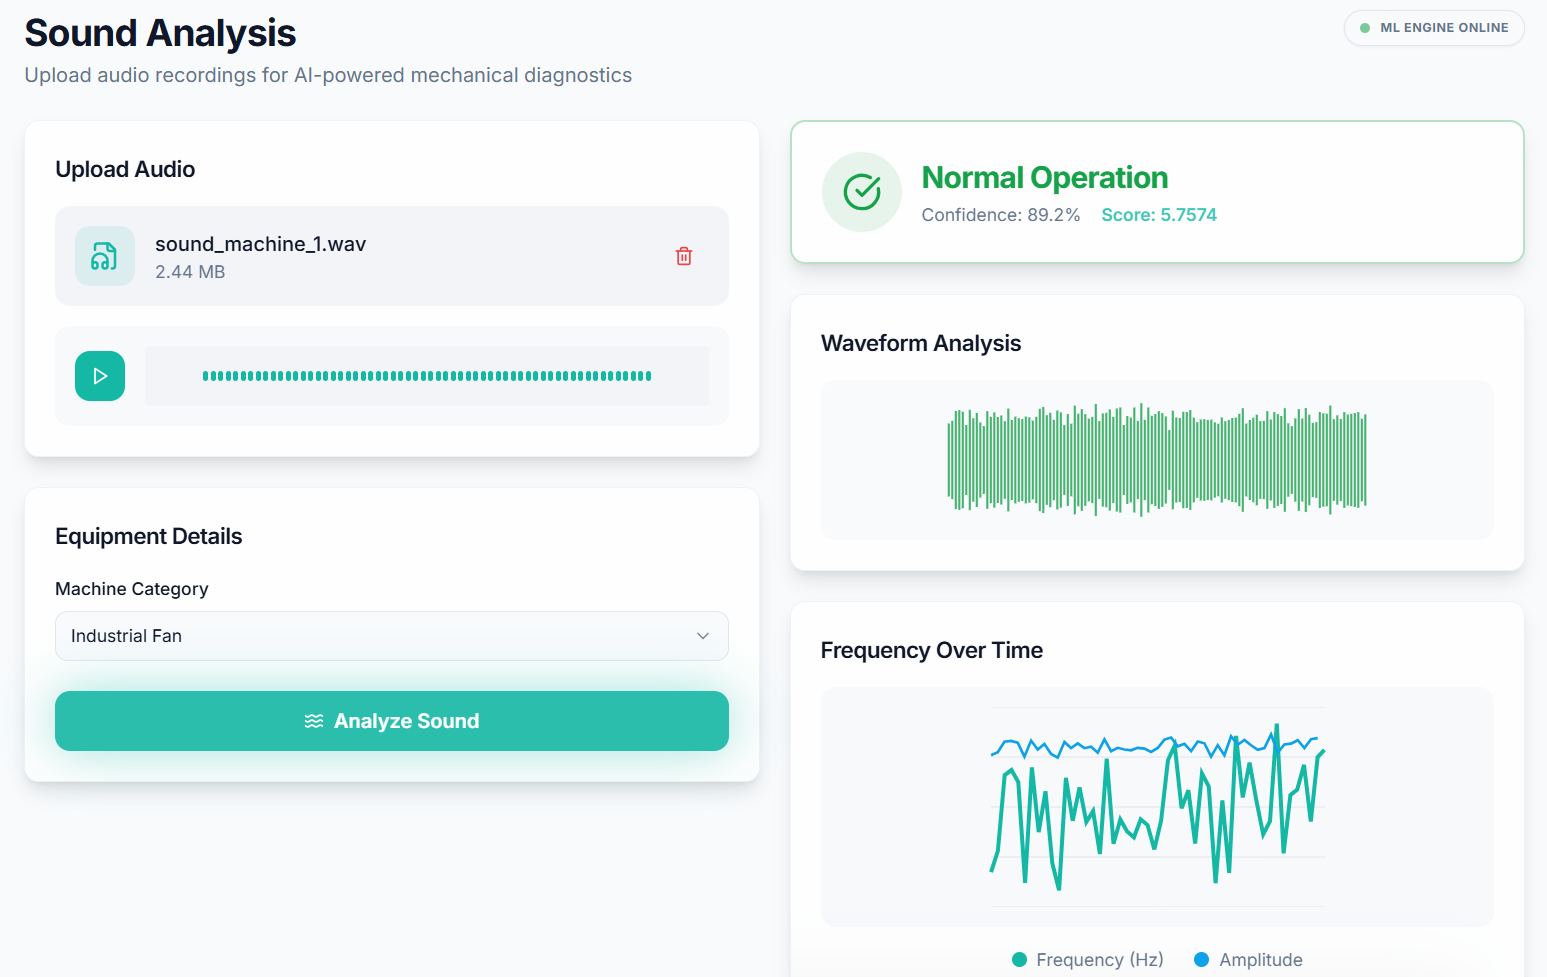
\includegraphics[width=\linewidth]{Test10.png}
  \caption{Normal --- Machine 1 (89.2\%)}
  \label{fig:test10}
\end{subfigure}
\hfill
\begin{subfigure}[b]{0.32\textwidth}
  \centering
  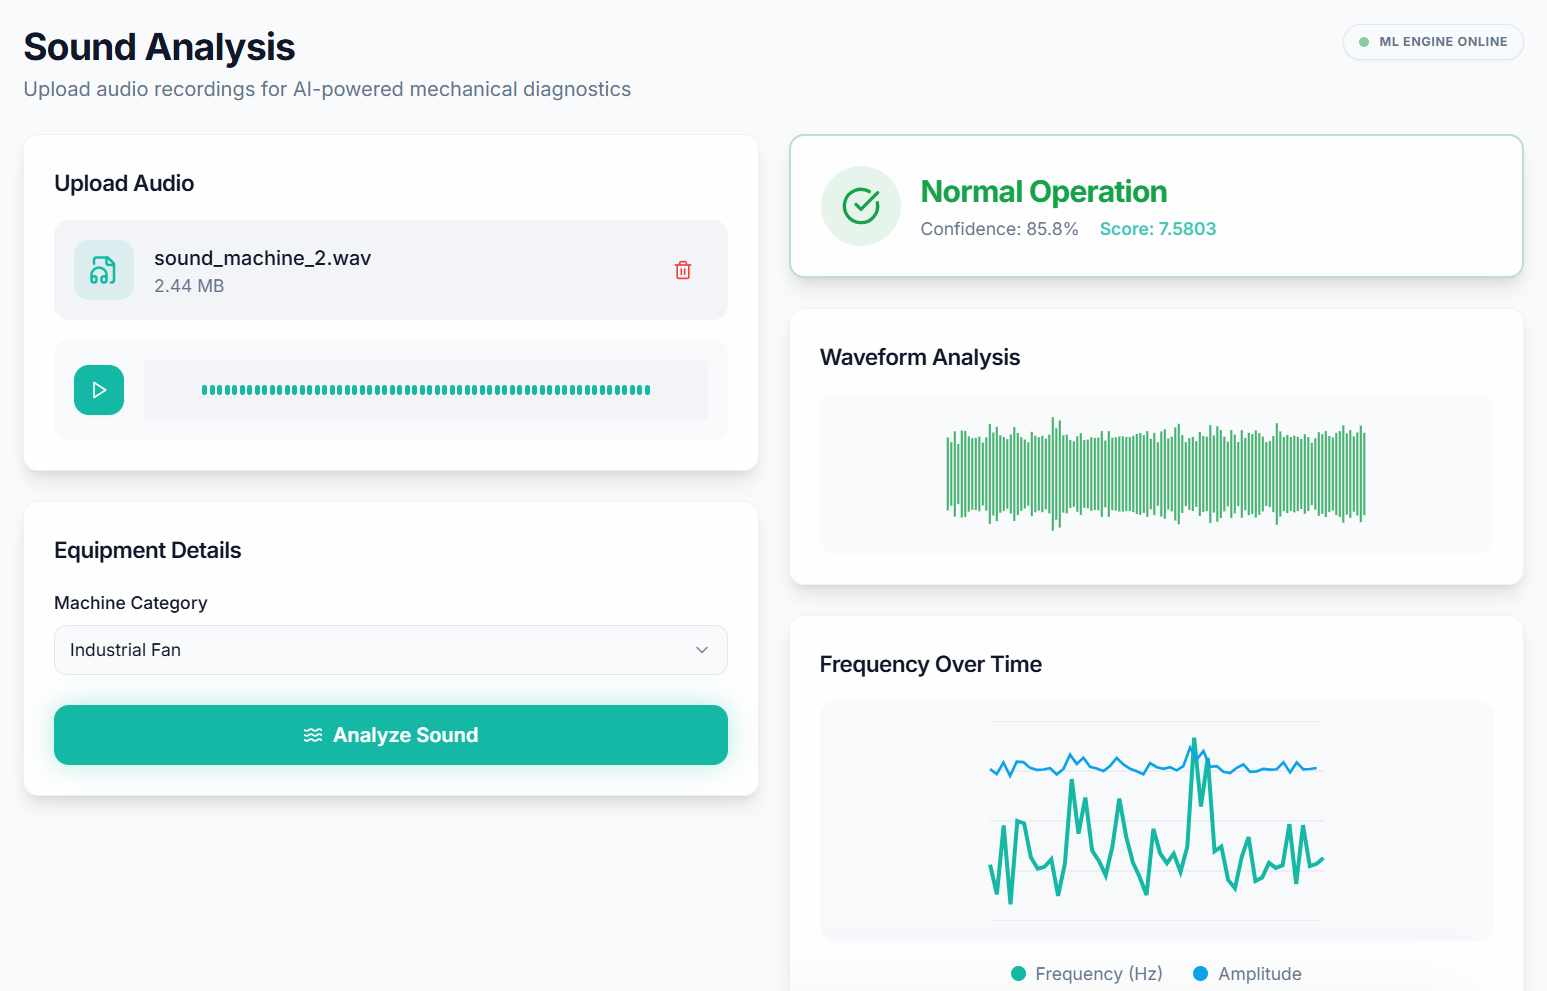
\includegraphics[width=\linewidth]{test11.png}
  \caption{Normal --- Machine 2 (85.8\%)}
  \label{fig:test11}
\end{subfigure}
\hfill
\begin{subfigure}[b]{0.32\textwidth}
  \centering
  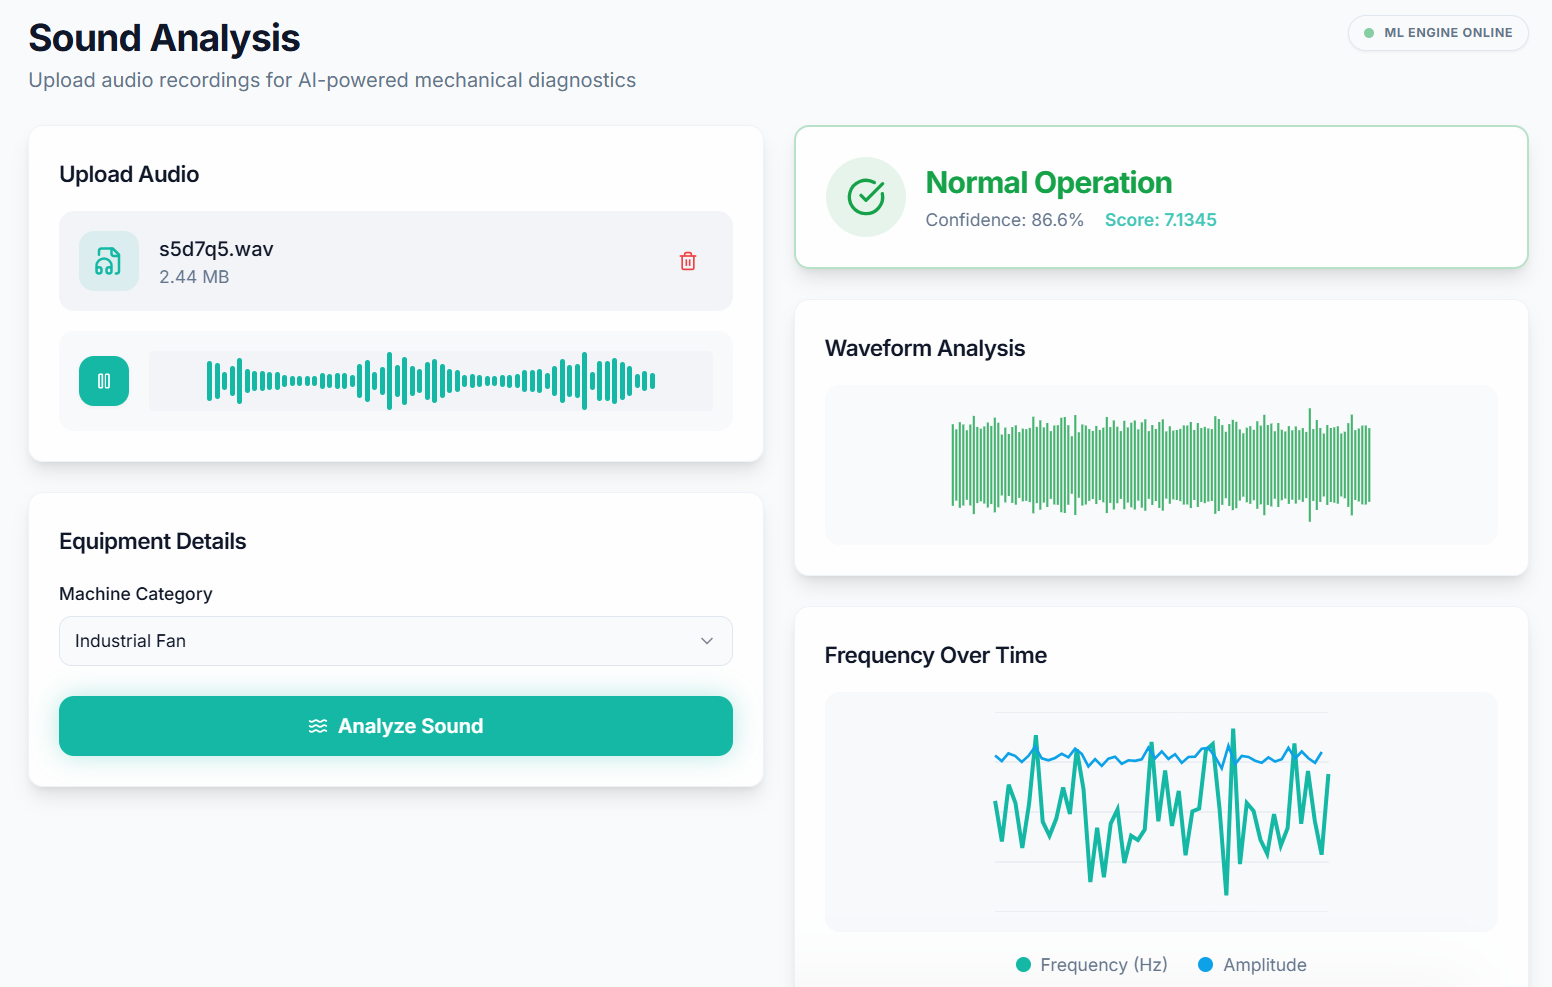
\includegraphics[width=\linewidth]{Test9.png}
  \caption{Normal --- s5d7q5 (86.6\%)}
  \label{fig:test9}
\end{subfigure}

\vspace{0.15cm}

\begin{subfigure}[b]{0.32\textwidth}
  \centering
  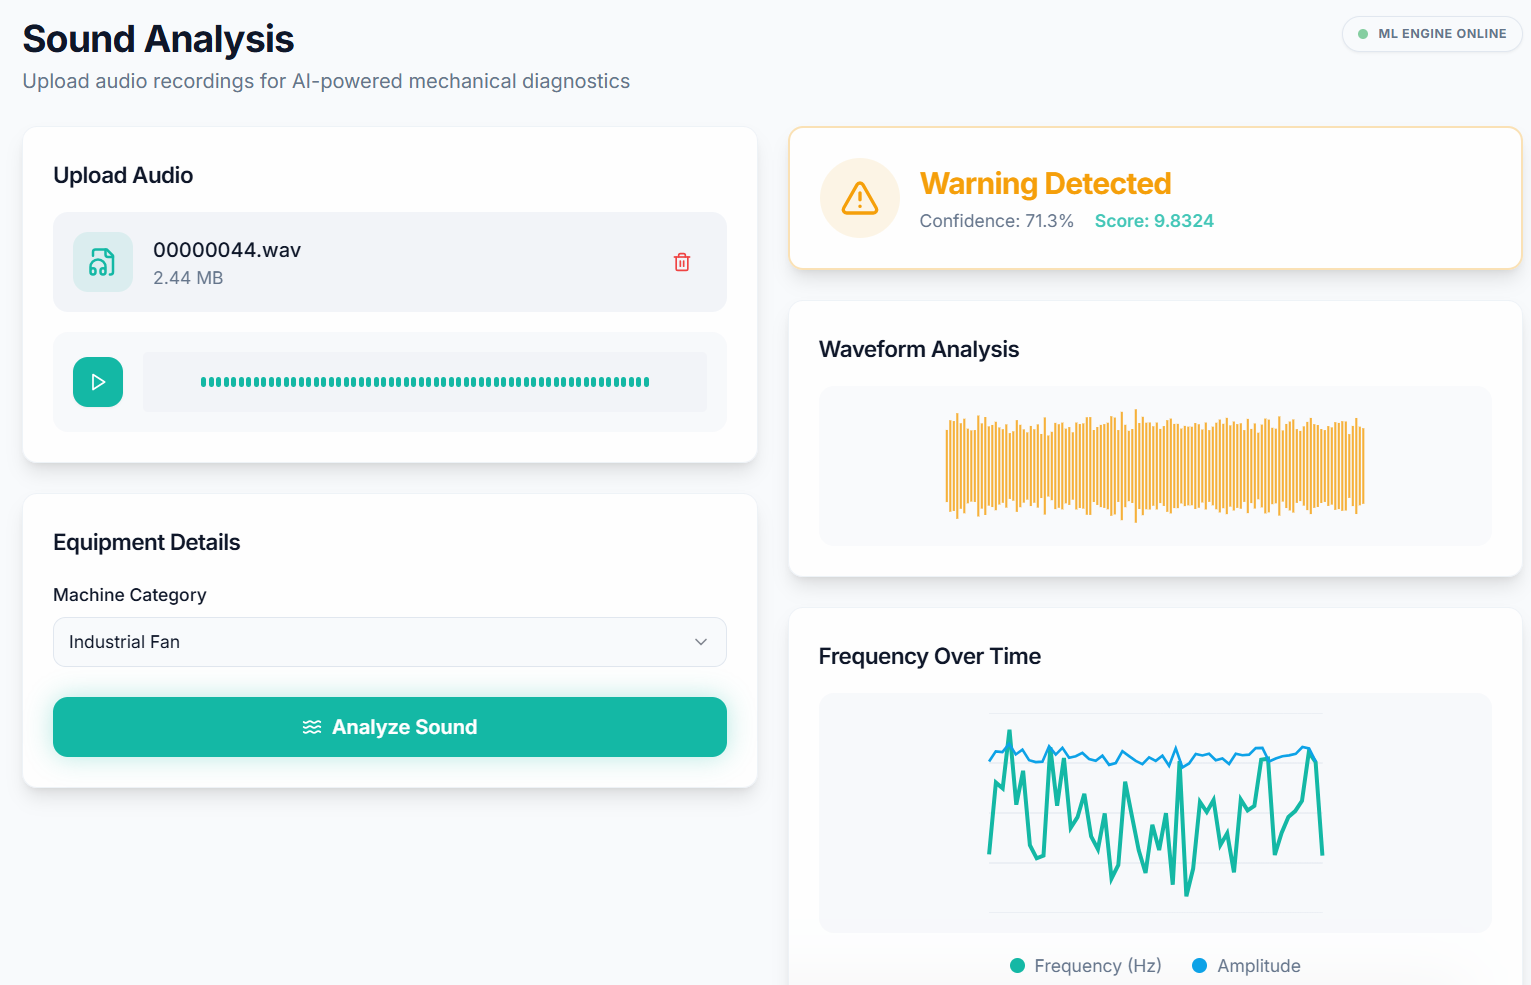
\includegraphics[width=\linewidth]{Test13.png}
  \caption{Warning --- 00000044 (71.3\%)}
  \label{fig:test13}
\end{subfigure}
\hfill
\begin{subfigure}[b]{0.32\textwidth}
  \centering
  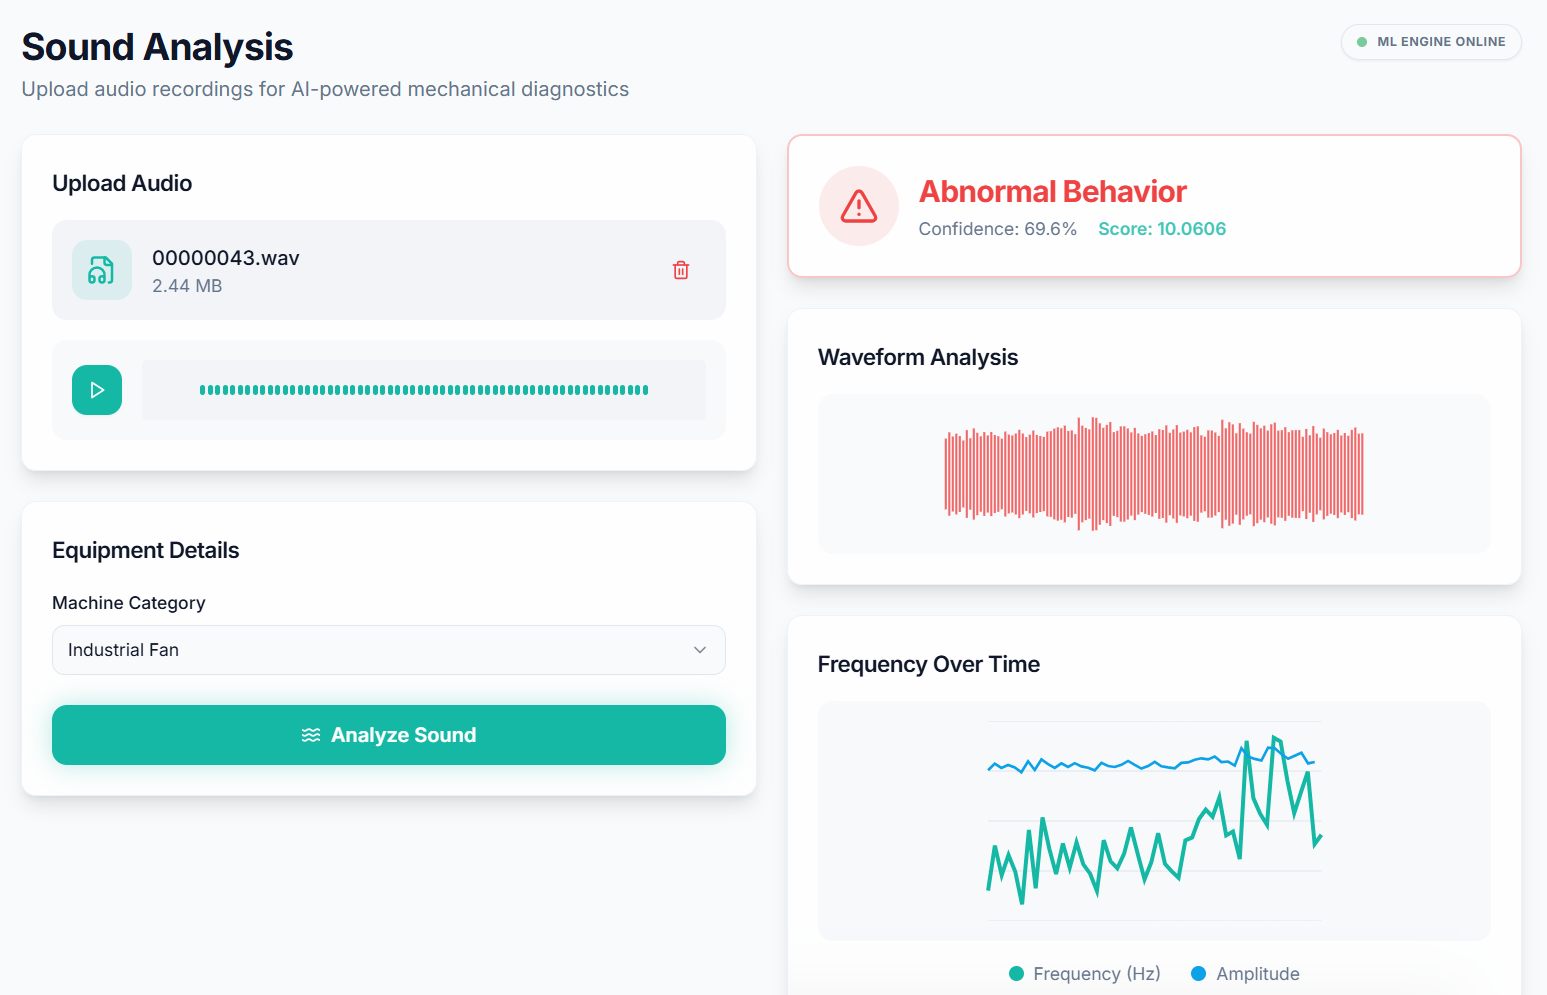
\includegraphics[width=\linewidth]{Test12.png}
  \caption{Abnormal --- 00000043 (69.6\%)}
  \label{fig:test12}
\end{subfigure}
\hfill
\begin{subfigure}[b]{0.32\textwidth}
  \centering
  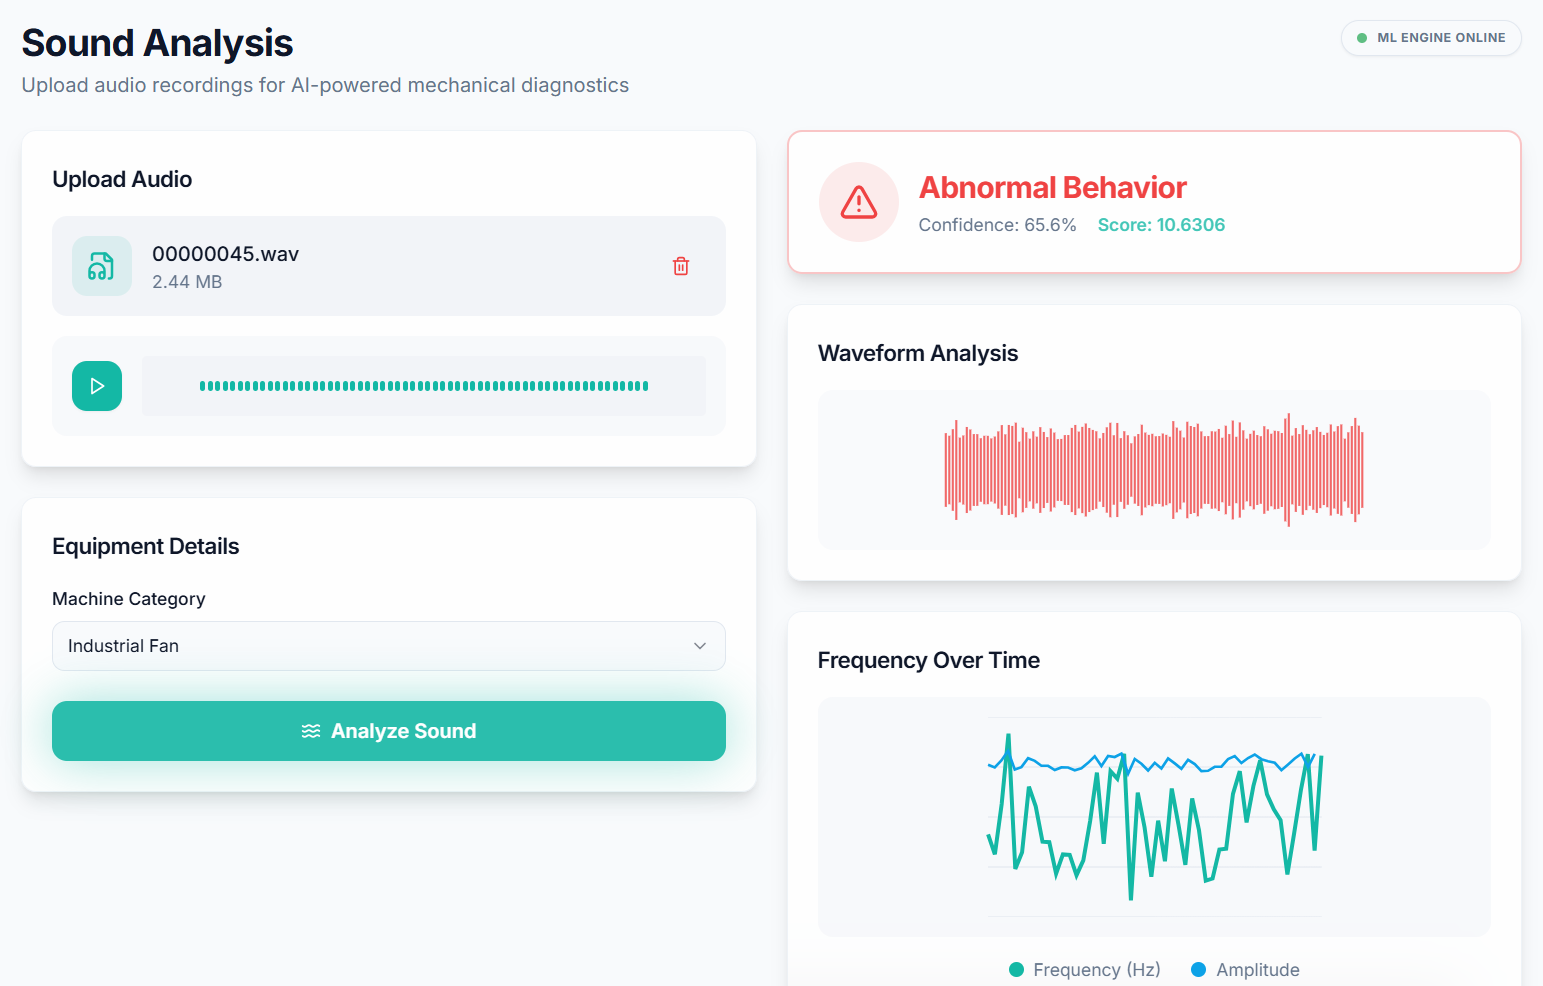
\includegraphics[width=\linewidth]{Test14.png}
  \caption{Abnormal --- 00000046 (62.5\%)}
  \label{fig:test14}
\end{subfigure}
\caption{Web Dashboard --- Sound Analysis Test Results}
\label{fig:test-results}
\end{figure}


% ══════════════════════════════════════════════════════════════════════════════
%  FOOTER
% ══════════════════════════════════════════════════════════════════════════════
\vfill
\begin{center}
\rule{0.5\textwidth}{0.4pt}\\[12pt]
\textit{\textcopyright\ 2026 Invictus-Team29, Faculty of Engineering, University of Peradeniya. All rights reserved.}\\[6pt]
\textit{This document has been prepared in accordance with IEEE Std 1063-2001,}\\
\textit{IEEE Standard for Software User Documentation.}
\end{center}

\end{document}
